\documentclass[a4paper,UKenglish]{lipics-v2018}
%This is a template for producing LIPIcs articles. 
%See lipics-manual.pdf for further information.
%for A4 paper format use option "a4paper", for US-letter use option "letterpaper"
%for british hyphenation rules use option "UKenglish", for american hyphenation rules use option "USenglish"
% for section-numbered lemmas etc., use "numberwithinsect"

\usepackage{listings}
\usepackage{color}
\usepackage{hyperref}
\usepackage{pdflscape}
\usepackage{enumerate}
\usepackage{hyperref}
\usepackage{graphicx}
\usepackage{lmodern}
\usepackage{url}
\usepackage{multirow}
\usepackage{amssymb}
\usepackage{xcolor}
\usepackage[normalem]{ulem}
\usepackage{tabularx}
\usepackage{adjustbox}
%% Some recommended packages.
\usepackage{booktabs}   
\usepackage{subcaption} 

\definecolor{mygreen}{rgb}{0.0, 0.5, 0.0}
\definecolor{myred}{rgb}{0.5,0.0,0.2}
\definecolor{LightGray}{gray}{0.9}

\newcommand{\greencheck}{{\color{mygreen}\checkmark}}
\newcommand{\redcross}{{\color{myred}$\times$}}




%*************************************************
% @(#)$Id: jml-listings.tex,v 1.6 2007/06/25 22:37:23 leavens Exp $
%
% Copyright (C) 2006 Iowa State University
%
% This file is part of JML
%
% JML is free software; you can redistribute it and/or modify
% it under the terms of the GNU General Public License as published by
% the Free Software Foundation; either version 2, or (at your option)
% any later version.
%
% JML is distributed in the hope that it will be useful,
% but WITHOUT ANY WARRANTY; without even the implied warranty of
% MERCHANTABILITY or FITNESS FOR A PARTICULAR PURPOSE.  See the
% GNU General Public License for more details.
%
% You should have received a copy of the GNU General Public License
% along with JML; see the file COPYING.  If not, write to
% the Free Software Foundation, 675 Mass Ave, Cambridge, MA 02139, USA.
%
% A JML listings environment.
%
% AUTHOR: Gary T. Leavens
%
% requires listings i.e., do \usepackage{listings} first
%
% This file is set up to be used via % @(#)$Id: jml-listings.tex,v 1.6 2007/06/25 22:37:23 leavens Exp $
%
% Copyright (C) 2006 Iowa State University
%
% This file is part of JML
%
% JML is free software; you can redistribute it and/or modify
% it under the terms of the GNU General Public License as published by
% the Free Software Foundation; either version 2, or (at your option)
% any later version.
%
% JML is distributed in the hope that it will be useful,
% but WITHOUT ANY WARRANTY; without even the implied warranty of
% MERCHANTABILITY or FITNESS FOR A PARTICULAR PURPOSE.  See the
% GNU General Public License for more details.
%
% You should have received a copy of the GNU General Public License
% along with JML; see the file COPYING.  If not, write to
% the Free Software Foundation, 675 Mass Ave, Cambridge, MA 02139, USA.
%
% A JML listings environment.
%
% AUTHOR: Gary T. Leavens
%
% requires listings i.e., do \usepackage{listings} first
%
% This file is set up to be used via % @(#)$Id: jml-listings.tex,v 1.6 2007/06/25 22:37:23 leavens Exp $
%
% Copyright (C) 2006 Iowa State University
%
% This file is part of JML
%
% JML is free software; you can redistribute it and/or modify
% it under the terms of the GNU General Public License as published by
% the Free Software Foundation; either version 2, or (at your option)
% any later version.
%
% JML is distributed in the hope that it will be useful,
% but WITHOUT ANY WARRANTY; without even the implied warranty of
% MERCHANTABILITY or FITNESS FOR A PARTICULAR PURPOSE.  See the
% GNU General Public License for more details.
%
% You should have received a copy of the GNU General Public License
% along with JML; see the file COPYING.  If not, write to
% the Free Software Foundation, 675 Mass Ave, Cambridge, MA 02139, USA.
%
% A JML listings environment.
%
% AUTHOR: Gary T. Leavens
%
% requires listings i.e., do \usepackage{listings} first
%
% This file is set up to be used via \input{jml-listings}.
% If you want, you could make a version that is a style file,
% but then change \lstdefinelanguage to \lst@definelanguage below.
%
\lstdefinelanguage[JML]{Java}[]{Java}%
       {% C++ style comments have to start with a blank!
        comment=[l]{//\ },
        % And C-style comments must also start with a blank or star!
        morecomment=[s]{/*\ }{*/},
        morecomment=[s]{/**}{*/},
        % sensitive=true, % inherited
        % Add JML keywords as level 1 keywords, so can typeset differently
        classoffset=1,
        % And here are all the wonderful JML keywords
        morekeywords={abrupt_behavior,abrupt_behaviour,
         accessible,accessible_redundantly,also,assert,assert_redundantly,
         assignable,assignable_redundantly,assume,assume_redundantly,
         axiom,behavior,behaviour,breaks,breaks_redundantly,
         callable,callable_redundantly,captures,captures_redundantly,
         choose,choose_if,codett,code_bigint_math,code_java_math,
         code_safe_math,constraint,constraint_redundantly,constructor,
         continues,continues_redundantly,decreases,decreases_redundantly,
         decreasing,decreasing_redundantly,diverges,diverges_redundantly,
         duration,duration_redundantly,ensures,ensures_redundantly,
         example,exceptional_behavior,exceptional_behaviour,
         exceptional_example,exsures,exsures_redundantly,extract,field,
         forall,for_example,ghost,helper,hence_by,hence_by_redundantly,
         implies_that,in,in_redundantly,initializer,initially,instance,
         invariant,invariant_redundantly,loop_invariant,
         loop_invariant_redundantly,maintaining,maintaining_redundantly,
         maps,maps_redundantly,measured_by,measured_by_redundantly,method,
         model,model_program,modifiable,modifiable_redundantly,modifies,
         modifies_redundantly,monitored,monitors_for,non_null,
         normal_behavior,normal_behaviour,normal_example,nowarn,
         nullable,nullable_by_default,old,or,post,post_redundantly,
         pre,pre_redundantly,pure,readable,refine,refines,refining,represents,
         represents_redundantly,requires,requires_redundantly,
         returns,returns_redundantly,sett,signals,signals_only,
         signals_only_redundantly,signals_redundantly,spec_bigint_math,
         spec_java_math,spec_protected,spec_public,spec_safe_math,
         static_initializer,uninitialized,unreachable,weakly,
         when,when_redundantly,working_space,working_space_redundantly,
         writable
        },
        % keywords from the universe type system
        morekeywords={rep,peer,readonly},
        % keywords from the AspectJ type system
        morekeywords={aspect, privileged, pointcut, before, after, returning, throwing, around,
        proceed, call, execution, target, this, args, thisJoinPoint,
        within, cflow, declare, precedence, parents},
         % keywords from the @AspectJ type system
        morekeywords={@Aspect, @Pointcut, @Before, @AfterReturning, @AfterThrowing, @After, @InterfaceXCS},
        % keywords from the @AspectJML type system
        morekeywords={@XCS},
        % typeset everything that starts with a backslash as a keyword
        % BUG: this doesn't allow typesetting these keywords differently
        keywordsprefix=\\,
        otherkeywords={<:,<-,->,..,<==,==>,<==>,<=!=>},
        classoffset=0 % restore default class for keywords
}
.
% If you want, you could make a version that is a style file,
% but then change \lstdefinelanguage to \lst@definelanguage below.
%
\lstdefinelanguage[JML]{Java}[]{Java}%
       {% C++ style comments have to start with a blank!
        comment=[l]{//\ },
        % And C-style comments must also start with a blank or star!
        morecomment=[s]{/*\ }{*/},
        morecomment=[s]{/**}{*/},
        % sensitive=true, % inherited
        % Add JML keywords as level 1 keywords, so can typeset differently
        classoffset=1,
        % And here are all the wonderful JML keywords
        morekeywords={abrupt_behavior,abrupt_behaviour,
         accessible,accessible_redundantly,also,assert,assert_redundantly,
         assignable,assignable_redundantly,assume,assume_redundantly,
         axiom,behavior,behaviour,breaks,breaks_redundantly,
         callable,callable_redundantly,captures,captures_redundantly,
         choose,choose_if,codett,code_bigint_math,code_java_math,
         code_safe_math,constraint,constraint_redundantly,constructor,
         continues,continues_redundantly,decreases,decreases_redundantly,
         decreasing,decreasing_redundantly,diverges,diverges_redundantly,
         duration,duration_redundantly,ensures,ensures_redundantly,
         example,exceptional_behavior,exceptional_behaviour,
         exceptional_example,exsures,exsures_redundantly,extract,field,
         forall,for_example,ghost,helper,hence_by,hence_by_redundantly,
         implies_that,in,in_redundantly,initializer,initially,instance,
         invariant,invariant_redundantly,loop_invariant,
         loop_invariant_redundantly,maintaining,maintaining_redundantly,
         maps,maps_redundantly,measured_by,measured_by_redundantly,method,
         model,model_program,modifiable,modifiable_redundantly,modifies,
         modifies_redundantly,monitored,monitors_for,non_null,
         normal_behavior,normal_behaviour,normal_example,nowarn,
         nullable,nullable_by_default,old,or,post,post_redundantly,
         pre,pre_redundantly,pure,readable,refine,refines,refining,represents,
         represents_redundantly,requires,requires_redundantly,
         returns,returns_redundantly,sett,signals,signals_only,
         signals_only_redundantly,signals_redundantly,spec_bigint_math,
         spec_java_math,spec_protected,spec_public,spec_safe_math,
         static_initializer,uninitialized,unreachable,weakly,
         when,when_redundantly,working_space,working_space_redundantly,
         writable
        },
        % keywords from the universe type system
        morekeywords={rep,peer,readonly},
        % keywords from the AspectJ type system
        morekeywords={aspect, privileged, pointcut, before, after, returning, throwing, around,
        proceed, call, execution, target, this, args, thisJoinPoint,
        within, cflow, declare, precedence, parents},
         % keywords from the @AspectJ type system
        morekeywords={@Aspect, @Pointcut, @Before, @AfterReturning, @AfterThrowing, @After, @InterfaceXCS},
        % keywords from the @AspectJML type system
        morekeywords={@XCS},
        % typeset everything that starts with a backslash as a keyword
        % BUG: this doesn't allow typesetting these keywords differently
        keywordsprefix=\\,
        otherkeywords={<:,<-,->,..,<==,==>,<==>,<=!=>},
        classoffset=0 % restore default class for keywords
}
.
% If you want, you could make a version that is a style file,
% but then change \lstdefinelanguage to \lst@definelanguage below.
%
\lstdefinelanguage[JML]{Java}[]{Java}%
       {% C++ style comments have to start with a blank!
        comment=[l]{//\ },
        % And C-style comments must also start with a blank or star!
        morecomment=[s]{/*\ }{*/},
        morecomment=[s]{/**}{*/},
        % sensitive=true, % inherited
        % Add JML keywords as level 1 keywords, so can typeset differently
        classoffset=1,
        % And here are all the wonderful JML keywords
        morekeywords={abrupt_behavior,abrupt_behaviour,
         accessible,accessible_redundantly,also,assert,assert_redundantly,
         assignable,assignable_redundantly,assume,assume_redundantly,
         axiom,behavior,behaviour,breaks,breaks_redundantly,
         callable,callable_redundantly,captures,captures_redundantly,
         choose,choose_if,codett,code_bigint_math,code_java_math,
         code_safe_math,constraint,constraint_redundantly,constructor,
         continues,continues_redundantly,decreases,decreases_redundantly,
         decreasing,decreasing_redundantly,diverges,diverges_redundantly,
         duration,duration_redundantly,ensures,ensures_redundantly,
         example,exceptional_behavior,exceptional_behaviour,
         exceptional_example,exsures,exsures_redundantly,extract,field,
         forall,for_example,ghost,helper,hence_by,hence_by_redundantly,
         implies_that,in,in_redundantly,initializer,initially,instance,
         invariant,invariant_redundantly,loop_invariant,
         loop_invariant_redundantly,maintaining,maintaining_redundantly,
         maps,maps_redundantly,measured_by,measured_by_redundantly,method,
         model,model_program,modifiable,modifiable_redundantly,modifies,
         modifies_redundantly,monitored,monitors_for,non_null,
         normal_behavior,normal_behaviour,normal_example,nowarn,
         nullable,nullable_by_default,old,or,post,post_redundantly,
         pre,pre_redundantly,pure,readable,refine,refines,refining,represents,
         represents_redundantly,requires,requires_redundantly,
         returns,returns_redundantly,sett,signals,signals_only,
         signals_only_redundantly,signals_redundantly,spec_bigint_math,
         spec_java_math,spec_protected,spec_public,spec_safe_math,
         static_initializer,uninitialized,unreachable,weakly,
         when,when_redundantly,working_space,working_space_redundantly,
         writable
        },
        % keywords from the universe type system
        morekeywords={rep,peer,readonly},
        % keywords from the AspectJ type system
        morekeywords={aspect, privileged, pointcut, before, after, returning, throwing, around,
        proceed, call, execution, target, this, args, thisJoinPoint,
        within, cflow, declare, precedence, parents},
         % keywords from the @AspectJ type system
        morekeywords={@Aspect, @Pointcut, @Before, @AfterReturning, @AfterThrowing, @After, @InterfaceXCS},
        % keywords from the @AspectJML type system
        morekeywords={@XCS},
        % typeset everything that starts with a backslash as a keyword
        % BUG: this doesn't allow typesetting these keywords differently
        keywordsprefix=\\,
        otherkeywords={<:,<-,->,..,<==,==>,<==>,<=!=>},
        classoffset=0 % restore default class for keywords
}

%\lstset{basicstyle=\ttfamily, keywordstyle=\bfseries, stringstyle=\ttfamily, mathescape=true, language={[JML]Java}}

\lstset{showspaces=false,
  showtabs=false,
  commentstyle=\color{mygreen}\bfseries,
  keywordstyle=\color{myred}\bfseries,
  stringstyle=\color{blue},
  language=Java,
  basicstyle=\ttfamily,
  showstringspaces=false,
}

\definecolor{darkgrey}{rgb}{0.70, 0.70, 0.70}
\definecolor{lightgrey}{rgb}{0.80, 0.80, 0.80}
\newcommand{\shd}[1]{\colorbox{lightgrey}{#1}}
\newcommand{\shdk}[1]{\colorbox{darkgrey}{#1}}
\newcommand{\jmloktool}[1]{\textsc{JmlOk2}}
\newcommand{\contractjdoc}[1]{\textsc{ContractJDoc}}
\newcommand{\contractjdocCompiler}[1]{\textsc{ajmlc-contractjdoc}}

%commands for constant values
\newcommand{\totalClauses}[1]{3,993}
\newcommand{\totalPre}[1]{1,952}
\newcommand{\totalPost}[1]{2,029}
\newcommand{\totalInv}[1]{19}
\newcommand{\totalCode}[1]{190,655}
\newcommand{\totalSystems}[1]{six}

% respondants of our survey
\newcommand{\surveyRespondants}[1]{142}

\usepackage{microtype}%if unwanted, comment out or use option "draft"
\bibliographystyle{plainurl}

\title{Design-by-Contract Javadoc for API Documentation: Trade-offs between Automatic Checking and Understandability}

\titlerunning{Design-by-Contract Javadoc for API Documentation}%optional, please use if title is longer than one line

\author{An Author}{An Institution}{author@authors.com}{}{}


% \author{Alysson Milanez}{Department of Systems and Computing, UFCG, Brazil}{alyssonfilgueira@copin.ufcg.edu.br}{}{}


% \author{Tiago Massoni}{Department of Systems and Computing, UFCG, Brazil}{massoni@dsc.ufcg.edu.br}{}{}

% \author{Henrique Reb\^{e}lo}{Informatics Center, UFPE, Brazil}{hemr@cin.ufpe.br}{}{}

% \author{Rohit Gheyi}{Department of Systems and Computing, UFCG, Brazil}{rohit@dsc.ufcg.edu.br}{}{}

% \author{Gary Leavens}{Department of Computer Science, UCF, USA}{leavens@cs.ucf.edu}{}{}

 \authorrunning{An Author}

% \Copyright{Alysson Milanez and Tiago Massoni and Henrique Reb\^{e}lo and Rohit Gheyi and Gary Leavens}%mandatory, please use full first names. LIPIcs license is "CC-BY";  http://creativecommons.org/licenses/by/3.0/


\subjclass{
\ccsdesc[500]{Software and its engineering~Software verification and validation, Software and its engineering~Domain specific languages}
}% mandatory: Please choose ACM 2012 classifications from https://www.acm.org/publications/class-2012 or https://dl.acm.org/ccs/ccs_flat.cfm . E.g., cite as "General and reference $\rightarrow$ General literature" or \ccsdesc[100]{General and reference~General literature}. 

\keywords{design-by-contract, documentation, runtime checking, Javadoc}

%\category{}%optional, e.g. invited paper
%\relatedversion{}%optional, e.g. full version hosted on arXiv, HAL, or other respository/website
%\supplement{TBD}%optional, e.g. related research data, source code, ... hosted on a repository like zenodo, figshare, GitHub, ...
%\funding{}%optional, to capture a funding statement, which applies to all authors. Please enter author specific funding statements as fifth argument of the \author macro.

%\acknowledgements{I want to thank \dots}%optional

\nolinenumbers %uncomment to disable line numbering
%\hideLIPIcs  %uncomment to remove references to LIPIcs series (logo, DOI, ...), e.g. when preparing a pre-final version to be uploaded to arXiv or another public repository

\begin{document}


\maketitle

\begin{abstract}
%context
Documenting public routines counts as a key benefit from applying the Design by Contract (DbC) methodology. 
In this context, DBC's pre- and post-conditions (public contracts) establish call conditions and expected results, respectively, which may be then checked at runtime for detecting invalid calls or nonconforming implementations.
%
% problem
It is well known, however, that programmers, despite this convenience, are resistant to use public contracts -- for Java programs, in particular, Javadoc natural text and tags are the dominant medium for documenting public routines.
As a result, verification assistance is unavailable.
%
% solution
In this paper, we report results from empirical studies on integrating contract expressions into Javadoc comments used as public contracts. 
For this purpose, we designed a small tag-based extension to Javadoc (\contractjdoc{}) to express pre- and post-conditions among other standard tags.
%
%studies
Studies consisted in (1) evaluating effectiveness and understandability of contract expressions within Javadoc, either for API users or developers, by means of a experimental study and a judgment survey, and in (2) investigating anomalies in Javadoc-rich open source systems that may arise when we manually formalize textual public contracts into contract expressions, then checking conformance at runtime.
%
%results
We observed higher quality of submissions as contracts were less formal, with satisfactory results when applying \contractjdoc with its semi-formal approach. Also, in terms of understandability, differences were discerned between different contract styles with variate levels of formality.
Given the fact that we found 391 anomalies between contracts and code in one large and four small open source Java systems, the results are promising in establishing hypotheses to the adoption of contract languages in mainstream development, by integrating informal and formal styles of documentation.
\end{abstract}

%(2) an empirical study
%with 24 programmers using three different documenting approaches, including
%\contractjdoc{}, whose results did not significantly differ, and (3) we surveyed 142 Java programmers regarding \contractjdoc{}'s
%readability in contrast to other two approaches (Javadoc and JML), in which
%results did not significantly differ for \contractjdoc{} and Javadoc, which is
%promising, since contracts are regarded as hard to read.


\section{Introduction}
\label{sec:introduction}

Java programmers tend to consider writing Javadoc comments as a good practice,
specially when these comments enhance public interfaces designed as third-party
libraries for client programs.
%
Despite its recognized value and practice in Java community, 
as discussed by ~\cite{liveAPI},
understanding how to use third-party libraries can be difficult.
This mainly occurs when the source of documentation is only natural language 
comments that can be incomplete and ambiguous. In addition, a well-known problem is that
documentation and implementation tend to diverge over time~\cite{Estler-etal14}; 
a Java programmer may forget to update the Javadoc documentation after performing 
an implementation change.

%
On the other hand, embedding contracts (with pre- and postconditions as executable assertions) has
long been advocated by formal methods pioneers to precisely express code behavior. 
However, only a small amount of code has such contracts~\cite{Polikarpova-etal09}. 
Part of the reason is notational, for example, in Java there is
no built-in support for contracts, besides \texttt{assert} statements.
To this end, we need an external contract framework like the Java Modeling Language (JML)~\cite{jml}
to express the full power of behavioral specifications.
%
There is evidence that programmers are more likely to use contracts in languages that support them
natively~\cite{Chalin06}, such as Microsoft's Code Contracts~\cite{codeContractsPaper} and Eiffel~\cite{eiffel}.
%
Another problem is that contracts expressed by
the existing contract languages may be useful for programmers (internal documentation), 
but it does not meet the needs of other
readers (separate/external documentation), such as third-party libraries~\cite{Leavens10,Parnas2011}. 
To use those libraries, a programmer should not need to look in the code to 
find out how to use it. 
%
Therefore, to maximize benefits, 
she must use the combination of such techniques (e.g., Javadoc and JML).

%
We propose a Javadoc-like language, called \contractjdoc{}, allowing Java programmers to add
contract specifications (pre- and postconditions), in a straightforward way, into Javadoc comments.
%
Only a few extensions are needed to allow contracts,
such as invariants.
%
To enable the power of contracts, the \contractjdoc{} compiler
translates the documented contracts into corresponding JML specifications. 
Then, these JML specifications, equipped with pre- and postconditions, are  
compiled into runtime conformance checks.
%

% how we evaluate
We evaluate our approach by performing three studies:
we first apply \contractjdoc{} to \totalSystems{} Javadoc-annotated open source
systems in order to analyse \contractjdoc{}'s applicability.
A number of previously-undetected inconsistencies between Javadoc and actual behaviour were found in some of the studied systems.
% \item %experimental study
Next, we report a study which observed 24 developers programming for Java interfaces with behaviour
documented by the conventional Javadoc, JML~\cite{jml}, and
\contractjdoc{}, within a controlled environment.
As result, developers found it easier to implement an interface with contracts
than writing a client for that interface. Also, in general pure Javadoc was straightforward to understand, but \contractjdoc{} performed better than JML, as we expected.
% \item %survey
Last, we investigate the readability of these three documentation approaches
for specifying behavior in a Java interface -- Javadoc, JML and \contractjdoc{}, by
means of a survey with 142 Java developers.
%results
Survey results did not significantly differ for \contractjdoc{} and Javadoc, which
is promising, as contracts are usually regarded as hard to read.

In summary, the main contributions of this paper are:
\begin{itemize}
\item A new approach for documenting source code -- \contractjdoc{} (Section~\ref{sec:approach});
\item A case study applying \contractjdoc{} to \totalSystems{} Javadoc-annotated open source
systems (Section~\ref{sec:caseStudy});
\item An empirical study with 24 developers programming for Java interfaces with behavior
documented by the conventional Javadoc, JML, and \contractjdoc{} (Section~\ref{sec:experiment});
\item A comprehensibility survey with 142 Java developers investigating the
readability of three documentation approaches for specifying behavior in a Java
interface: Javadoc, JML and \contractjdoc{} (Section~\ref{sec:survey}).
\end{itemize}


\subsection{Research Questions}
\label{sec:researchQuestions}

%intro paragraph
This research work investigates what is the impact of integrating contract expressions with Javadoc comments in public interfaces, in terms of applicability and usability. We first examine the impact of diverse contract documentation approaches with tasks related to the specification of data structure interfaces; as a follow-up, we inquired developers regarding understandability of contract examples. Second, we emulate the application of contract expressions to Javadoc-rich open source systems and analyzed results from runtime checking. In particular, we intend to answer the following research questions:  

\noindent\emph{RQ1. What is the success rate of public interface implementors and users in tasks, using three forms of public interface contracts?}\\
We report and discuss results from a lab study with Java developers over development tasks involving a documented data structure interface.

  
\noindent\emph{RQ2. What are the perceived difficulty in using three forms of public interface contracts?}\\
By means of a lab study with assigned tasks and a developer survey, we discuss quantitative and qualitative reports from developers regarding the forms of contract expressions that are preferred for implementation tasks.


\noindent\emph{RQ3. Can we uncover inconsistencies in Java systems if using runtime-checkable contract expressions?}\\
We collected a few open source systems based on their use of Javadoc, applied contract expressions
to each system and evaluated results in terms of detected conformance errors. Also, we discuss the problems faced when replacing Javadoc comments by contract expressions in the described context.

%TO DO: ver se é interessante colocar contribuições aqui.
\section{Styles of Public Contracts}
\label{sec:example}

In this section, we discuss issues in specifying the behaviour of API interfaces. For concreteness, we provide Java examples.

\subsection{Javadoc and textual specifications}

%documentation in Javadoc - no invariant
Javadoc~\cite{javadoc-oracle} is the usual notation (and tool) for API specifications in Java; it includes special tags (with symbol \@) for structuring and pretty-printing code commentary.
The Java Platform API specification itself~\cite{java-spec}, for instance, employs Javadoc for specifying "contract[s] between callers and implementations."
In those terms, Javadoc may be a tool for applying the Design-by-Contract (DBC) methodology~\cite{dbc}, with its pre- and post-conditions around public methods, establishing the expected behaviour for each part (the contract). In the context of distributed software teams, for instance, this kind of documentation is of critical importance. 


%java interface
Consider the bank account API depicted in Figure~\ref{Fig-Javadoc-Bank}\footnote{we consider API the public members of a Java class, or a Java interface}. For simplicity, only method {\lstinline!withdraw!} is declared. Tag \lstinline!@param! includes, for parameter \lstinline!amt!, a description that suffices as a pre-condition for \lstinline!withdraw! callers. Likewise, tags \lstinline!@return! and \lstinline!@throws! document, respectively, a normal post-condition (if it works correctly) and a exceptional post-condition (if \lstinline!TransactionException! is thrown).


\begin{figure}
\centering
\begin{lstlisting}[basicstyle=\footnotesize\ttfamily,name=figxpi]
class BankAccount {
 // ...
 /**
  * @param amt  the amount value to withdraw, where
  *             'amt' must be greater than zero 
  * @return     current 'balance' after withdraw
  * @throws     TransactionException 'balance' 
  *             remains unchanged
  *
  */
 double withdraw(double amt) 
   throws TransactionException {...}
 // ...
}
\end{lstlisting}
\caption{Bank Account API Specification using Javadoc.}
\label{Fig-Javadoc-Bank}
\end{figure}


%natural langague
Contracts in such style use natural language. As a consequence, consistency between specifications and actual code behaviour cannot be automatically enforced, unless one maintains test cases in synchronicity with the Javadoc contracts. However, even test cases are hardly up-to-date to code changes~\cite{Hao2013}, so it is hard to imagine that would be applicable. 
Furthermore, the lack of formality leads to imprecision, ambiguity, and verbosity, potentially leading to program anomalies and faults.
This poses translation problems to use natural language description for automated tools, such as in testing or debugging.

On the other hand, using natural language does not require special training -- although training may be needed to effectively communicate
ideas about program behaviour -- and allows a high degree of freedom for documentation structuring. 


\subsection{Formal Contracts}


DBC is supported by contruction in a few programming languages (such as Eiffel~\cite{eiffel}), or by extensions (Java Modeling Language (JML)~\cite{jml} for Java and Code Contracts~\cite{codeContractsPaper} for .NET languages) in mainstream programming languages.
For Java, JML contracts may be defined as showed in the same API for a bank account, in Figure~\ref{Fig-JML-Bank}. Pre-conditions
are defined by the clause {\lstinline!requires!} and (normal) post-conditions by {\lstinline!ensures!}. The specification
denoted by the {\lstinline!signals!} clause
is an exceptional post-condition stating that {\lstinline!balance!} should be unchanged, when the exception \texttt{TransactionExcep\-tion} is thrown.

\begin{figure}
\begin{lstlisting}[basicstyle=\footnotesize\ttfamily,name=figxpi]
class BankAccount {
 double balance;

 //@ requires amt > 0 && amt <= balance;
 //@ ensures balance == \old(balance - amt);
 //@ ensures \result == balance;
 //@ signals (TransactionException) 
 //@   balance == \old(balance);
 double withdraw(double amt) 
   throws TransactionException {...}
 // ...
}
\end{lstlisting}
\caption{The JML specifications for the bank account.}
\label{Fig-JML-Bank}
\end{figure}

In this style, formal contracts for methods, unlike natural approaches, precisely describe what must be true when the method is called, what must be true when the method return or when it returns abnormally. A critical property of such contracts is that they are machine-checkable, either by assertion testing or static analysis\~cite{Chalin06}.
%In addition for object-oriented languages, contracts can describe object invariants that must hold for an object in all of its visible states -- in this paper,.
Nevertheless, using JML-like formal contracts might require some level of training, hence becoming, to some extent, hard to read and write, and hence is often used sparingly~\cite{Chalin06,Polikarpova-etal09,typeContracts}.
In addition, assuming the code in Figure~\ref{Fig-JML-Bank} is an API with no available code, the specification is needed to use the API. However, usually formal contracts are only available for the API implementors, thus becoming not useful for its clients~\cite{Parnas2011}.


%The Documentation Dilemma
It is clear that we face a dilemma with respect to program documentation. If we use JML to provide formal documentation for contracts, the result is a more precise documentation, with the possibility of automatic checks. However, also results in a less flexible documentation in terms of using natural language to structure it.
If we refer to a more flexible and informal documentation approach such as Javadoc, we face the lack of precision and potential ambiguity, even though Javadoc comments are more useful for third-party libraries users. This dilemma leads us to the following  inquiries: is it possible to have the best of both worlds, mixing informal documentation and contract specification within a unified framework? In this case, what would be the effect of using such approach to API usage and development? This paper tries to enhance evidence on DBC development and languages by focusing on those questions.

%In the following, we discuss how \contractjdoc{} provides means to combine the benefits
% and overcome the main limitations 
%of the existing documentation approaches discussed previously.
\section{A Javadoc Extension for Public Contracts}
\label{sec:approach}

%update to be more general
In order to perform studies on approaches for specifying public contracts, we propose \contractjdoc{}, a simple extension to the Javadoc-tagging systems with contracts. Its compilation system is built on the top of the AspectJML compiler~\cite{aspectjml}, providing support for runtime checking of the contracts.
\contractjdoc{} allows programmers to document \emph{contract expressions} amid Javadoc header for methods. With just a few new tags, in addition to the standard Javadoc tags, one can write contracts as Javadoc comments that are compiled to runtime checkable code. 
%The \contractjdoc{} approach fulfills the gap between informal documentation (as with Javadoc) and formal specification (such as JML~\cite{jml} or Code Contracts~\cite{codeContractsPaper}).

In the remaining of this section, we present, based on a running example, how \contractjdoc{} supports a mixed approach, which combines textual documentation with a limited set of formal features from the examples in Section~\ref{sec:example}.

\subsection{Language Extension Design}

The \contractjdoc{} tags act as traditional Javadoc tags,  embedded within block comments. 
The main idea is to allow a mix between the traditional Javadoc syntax and JML-like notation; 
JML seems apropriate in this context, since it is built over Java expressions, with exception of a few logical operators (such as \texttt{==>} -- implication).
Embedding contracts allows for contract expressions (e.g., pre-conditions) in the existing Javadoc comments
and making them machine discoverable through the use of
marker brackets within those comments.
%semantic-neutral
In this proposal, we consider the textual comments surrounding the formal expressions semantically neutral -- we assume the expression does not change its semantics. 

%benefits
The potential benefit of embedding contract expressions in a more natural setting for the developer is his/her ability to remain within a single artifact which is purpose-built for writing API specifications. 
This is specially true because the overwhelming majority of contracts that programmers write in
practice are short and simple~\cite{Estler-etal14,typeContracts}. For instance, in 75\% of Code Contracts~\cite{codeContractsPaper} projects, the written contracts are basic checks for the presence of data (e.g., non-null checks)~\cite{typeContracts}. In such scenarios, there is no additional effort in embedding such contracts in Javadoc comments using our \contractjdoc{} approach.

\subsubsection{Pre-conditions}
%Recall the precondition illustrated in Section~\ref{sec:example}. We discussed two ways to document such a precondition, a formal one in JML (see Figure~\ref{Fig-JML-Bank}) and an informal one with plain Javadoc comments (see Figure~\ref{Fig-Javadoc-Bank}).
In \contractjdoc, the pre-condition for method \lstinline!withdraw! from Section~\ref{sec:example} can be rewritten as the excerpt in Figure~\ref{fig:pre-example}.

\begin{figure}
\centering
\begin{lstlisting}[basicstyle=\footnotesize\ttfamily,name=figxpi, frame=lines, mathescape=true]
 /**
  * @param amt the amount value to withdraw, 
  *   where $\shd{[amt > 0 \&\& amt <= balance]}$
  */
 double withdraw(double amt) 
   throws TransactionException {...}
\end{lstlisting}
\caption{\texttt{withdraw}'s pre-condition.}
\label{fig:pre-example}
\end{figure}

%explain
Tag \lstinline!@param! documents parameter \lstinline!amt! of \lstinline!double! type.
Besides the usual comments, we have added a boolean expression
surrounded by brackets; these brackets indicate assertions internally to the \contractjdoc{} compiler, so the comments can be turned into an executable precondition checking.
An alternative (not showed) is to replace tag \lstinline!@param! by \lstinline!@requires! or \lstinline!@pre!. Both can be used to document a precondition constraint; the main difference is that they are not part of the standard Javadoc tagging system.

\subsubsection{Post-conditions}

We may use \contractjdoc{} for post-conditions as the example in Figure~\ref{fig:post-example}.


\begin{figure}
\centering
\begin{lstlisting}[basicstyle=\footnotesize\ttfamily,name=figxpi, frame=lines, mathescape=true]
 /**
  * @return amt the current balance after withdraw,
  *   that is $\shd{[@return == balance]}$
  * @throws TransactionException the 'balance' does
  *  not change, that is $\shd{[balance == @old(balance)]}$
  */
 double withdraw(double amt) 
   throws TransactionException {...}
\end{lstlisting}
\caption{\texttt{withdraw}'s post-condition.}
\label{fig:post-example}
\end{figure}

Tags \lstinline!@return! and \lstinline!@throws! document normal and exceptional post-conditions, respectively, with their respective expressions
expressed within brackets.
%Tag \lstinline!@return! appears again within the brackets. This inner is allowed (in \contractjdoc{}) and allows one
%to use the value of the method's  returns to write the contract regarding
%the normal postcondition. A similar tag, \lstinline!@result! derived from the JML syntax,
%can also be employed instead of the inner use of the \lstinline!@return! tag.
Tag \lstinline!@old! refers to expressions or fields in their pre-state, used only in post-conditions.

As with preconditions, \contractjdoc{} offers three tags for expressing postconditions.
For normal postconditions, similar JML-based tags \lstinline!@ensures! and \lstinline!@post! may be used instead of \lstinline!@return!.
For \lstinline!@throws! tag, the standard Javadoc offers a surrogate tag \lstinline!@exception!. 
Derived from JML, we can also employ \lstinline!@signals! to document and constrain exceptional behavior.

% \subsubsection{Documenting Invariants}

% Beyond the support for pre- and postconditions, \contractjdoc{} make the use of invariants also
% available by means of \texttt{@inv} tags.
% The format of writing is the same as those
% for pre- and postconditions.
% The difference is related to the semantics: while pre- and postconditions apply to a specific
% method, an invariant applies for all methods from a class. For invariants, we follow the
% semantics of the JML language. For more information, please refer
% to~\cite{jml}.
% The invariant contract, described in Section~\ref{sec:example}, can be written
% as follows:
% \begin{lstlisting}[basicstyle=\footnotesize\ttfamily,name=figxpi, frame=lines, mathescape=true]
% class BankAccount {
%  /**
%   * @inv The overall balance should be $\shd{[balance >= 0]}$
%   */
%  double balance;
%  //...
% }
% \end{lstlisting}
% Invariant declarations may be placed above the field
% declarations (as in the example), or  above the
% class declaration as a valid Javadoc block comment.

\subsection{Supporting Infrastructure}

The \contractjdoc{} compiler is based on the open source AspectJML/ajmlc compiler~\cite{aspectjml,ajmlc,Rebelo-etal08}.
Unlike the standard JML compiler jmlc~\cite{jmlc-compiler}, ajmlc presents code optimizations and improved error reporting~\cite{ajmlc}.
Also, AspectJML enables the modularization
of crosscutting contracts that can arise in standard
JML specifications~\cite{aspectjml}.

We adapted the front-end of the AspectJML/ajmlc compiler to convert/preprocess the \contractjdoc{} tags into the corresponding JML features, like pre- and post-conditions.
After conversion, the compilation occurs as usual and generates aspects to runtime checking the
contracts. See Figure~\ref{fig:compilerInfra}
for an overview of the compilation strategy.
First, source code with \contractjdoc{}
contract expressions goes through a tag processor and a type checker. Next, a runtime assertion aspect is generated, which is woven to the source code by the aspectj compiler, producing bytecode with assertions, amenable to runtime checking.


\begin{figure}[h]
\centering
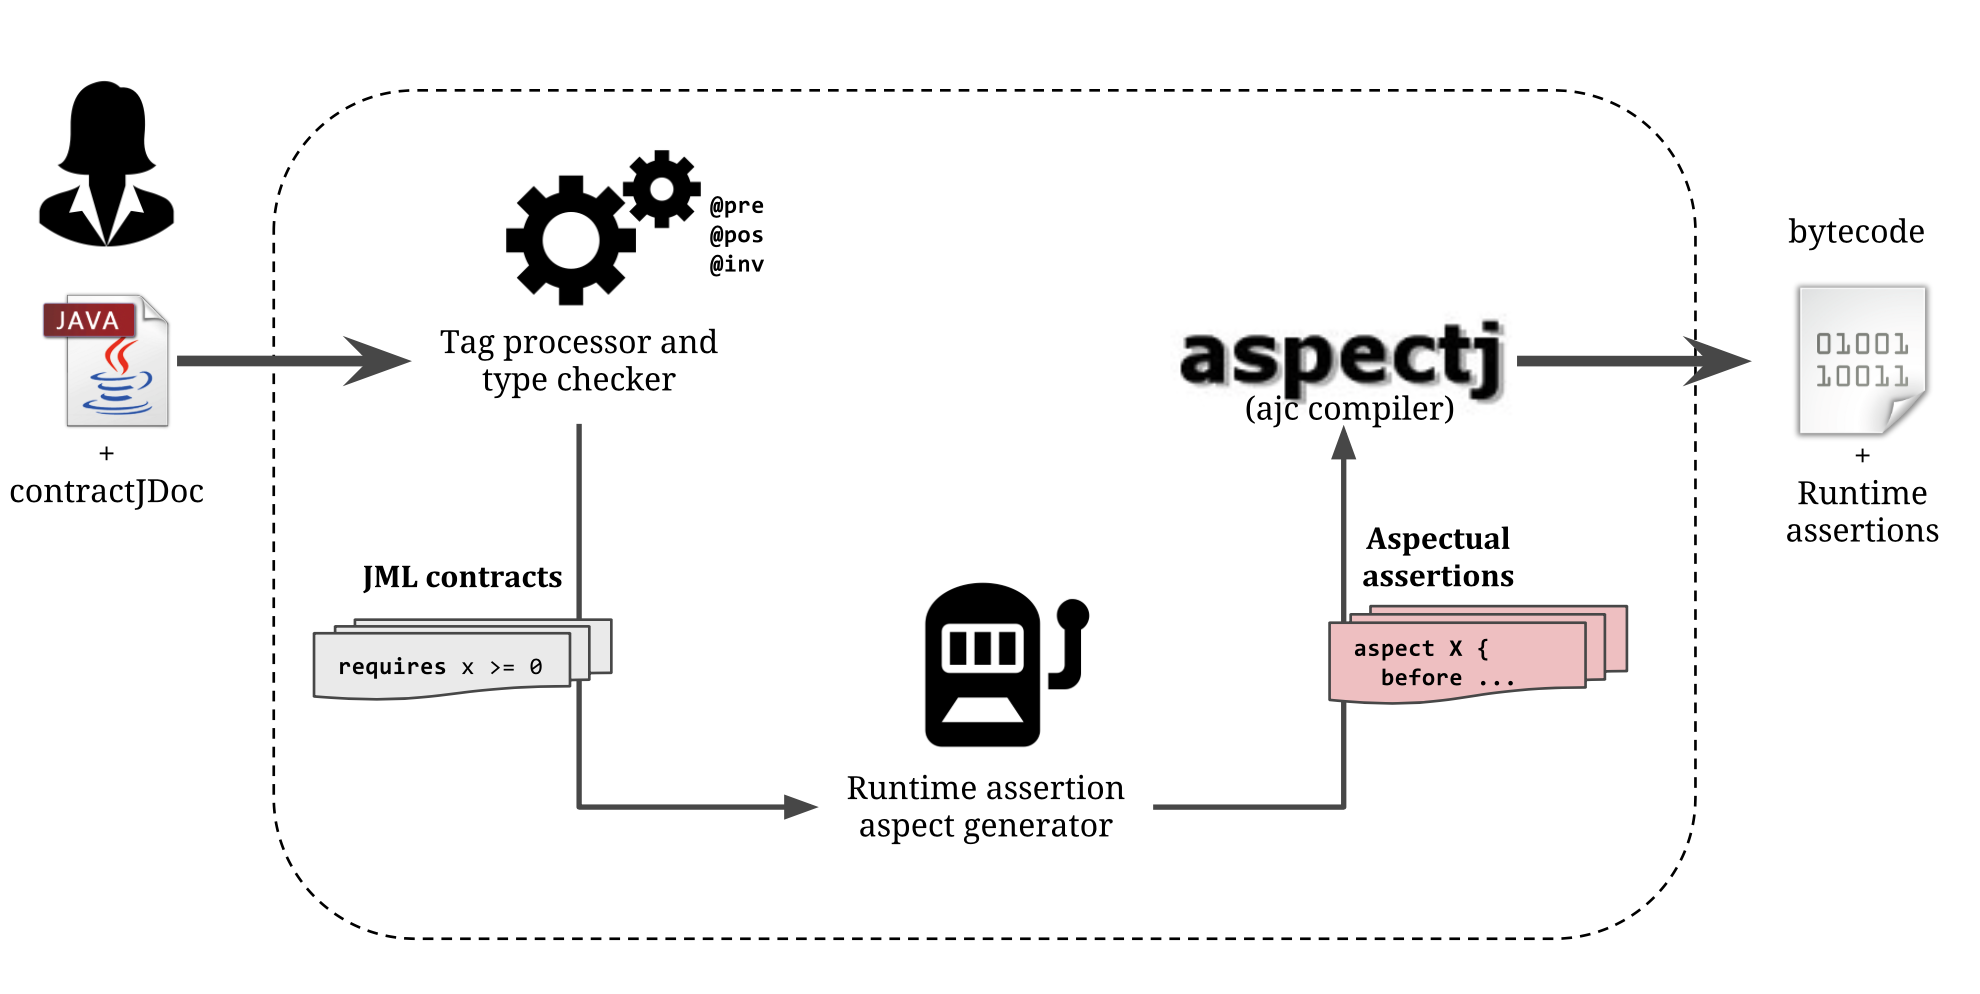
\includegraphics[width=1.0\textwidth]{figs/compilerInfra}
\caption{Compilation Infrastructure for ContractjDoc.}
\label{fig:compilerInfra}
\end{figure}


\section{Methodology}
\label{sec:researchDesign}

In the following subsections we discuss data collection and analysis for the performed studies. For naming the studies, we follow the terminology for Software Engineering research strategies from Stol and Fitzgerald~\cite{Stol2015}.


%nomenclatura

%Experimental simulation
%Judgement task
%Field Study


\subsection{Experimental Simulation}
\label{sec:experiment}

%GQM
In this study, we investigate the use of
external contract expressions -- in particular, \contractjdoc{}, as showed in Section\ref{sec:approach} -- in simulated programming tasks, with respect to applicability and understandability, from the point of view of Java developers. 

\subsubsection{Participants}
\label{sec:expPart}

%recruitment
We selected participants among professional developers assigned to projects in the context of an major R\&D Institute in Brazil. Recruitment was carried out by invitation; from estimated 150 invited professionals, 24 of them accepted the call and then, later, received the assignment by e-mail. The only requirement was previous experience with Java. From the 24 recruited developers, 10 of them had computer science (or related) degrees, while the remaining were carrying out undergraduate studies in the field. 

%number of participants
Although the number of participants may seem too small for generalizing any conclusions, we expect the observations to be considered as an exploratory theory to be checked by future studies with larger samples.
For experimental simulations, our participant set is within the expected size~\cite{}.


\subsubsection{Study Design}
\label{sec:studyDesign}

%factors
Our experiment was designed to assess the effect of a given documentation approach on implementation tasks which depend on documented APIs. 
%factor 1
Participants are assigned to use a single documentation approach (Factor 1) from the following: plain Javadoc natural language, our Javadoc extension and formal contracts. Table~\ref{tab:factorsEmpStudy} displays the treatments for those two factors.
%factor 2
For each of those approaches, two kinds of task are considered (Factor 2): a \textit{Supplier} task, in which the participant must program the implementation of a Java API class, and a \textit{Client} task, which demands development of a client code for the API.
%factor 3
An additional variation we included regards the particular API assigned to an arbitrary participant (Factor 3): \textit{Stack} or \textit{Queue}. We chose to use simple and well-known interfaces trying to avoid the confounding effect that lack of knowledge could bring to the study.


\begin{table}[ht]
\caption{Factors and treatments of the empirical study.}
\label{tab:factorsEmpStudy}
\centering
\begin{tabular}{ll} \toprule
\bfseries Factors & \bfseries Treatments \\
\hline

\multirow{2}{*}{\textbf{Task}} & Client \\
& Supplier \\ \hline 

\multirow{3}{*}{\textbf{Approach}} & Javadoc extension \\
 & Javadoc \\
& formal contracts \\ \bottomrule
\end{tabular}
\end{table}

%design
We use a factorial design~\cite{wohlin}, randomly assigning participants to each combination of treatments; each triple
$<$approach, task, API$>$ is called a trial.
Since there are three documenting approaches, two tasks and two Java interfaces, there are 12 possible trials, so each of them was carried out by two participants, resulting in a balanced design. 
The assignment Participant -- Trial is performed by using a
completely randomized design in order to minimize bias.


\subsubsection{Experimental Procedure}
\label{sec:expProcedure}

The experiment was performed offline, i.e., participants received the experimental package via an online Survey
platform\footnote{An instance of the platform used is
available online: \url{https://www.formpl.us/form/5671648952844288}} that we use to collect the results.
% double blind process 
% An example of survey sent to the
% participants can be found online.\footnote{\url{https://goo.gl/forms/ySTsYfKSRcotLayk1}} 

The experimental package consisted of (i) a statement of consent, (ii) a pretest
questionnaire, (iii) instructions and materials to perform the experiment, and (iv) a post-test
questionnaire. 
The instructions contained what we expected from the participants: they were asked to perform an implementation task (a supplier or a client code) for the
provided API. Each participant received one of the following tasks: create a supplier code for
an API or a client code using the API methods.
We also asked each participant to fulfill a
pre-study questionnaire reporting their programming experience (with respect to Java and contract-based programming experience). 
%After filling in the questionnaire, we randomly assign a task.

During the assignment, participants were allowed to review additional information -- part of the experimental package -- about the assigned documentation approach. 
%the tasks 1
For \textit{Supplier} tasks, participants should have implemented variations of well-known stack or queue operations whose intended behaviour was documented as \contractjdoc{} expressions. The following example shows the contract for \lstinline!Queue.add!, written in plain Javadoc commentary.
%example
\begin{lstlisting}[basicstyle=\footnotesize\ttfamily,name=figxpi, frame=lines, mathescape=true]
/**
   * Inserts the specified account into the queue 
   * if it is possible to do so 
   * immediately without violating capacity 
   * restrictions, returning true upon 
   * success and throwing an AccountQueueException 
   * if no space is currently available.
   * @param acc - the account to be added. 
   *     Must not be null.
   * @return true if the operation occurs with success.
   * @throws AccountQueueException - if the queue is 
   *     full or the account is null.
   */
  public boolean add(Account acc) throws AccountQueueException;
\end{lstlisting}

%the tasks 2
Differently, \textit{Client} tasks were carried out based on textual descriptions, although any call to API should fulfill its external contracts, also presented using one of the three documentation options. Implementation of the API were provided as binaries, so, as a result, participants were not given access to the source code.
%post-study
Before sending the results back, we asked the participants to answer a a post-experiment questionnaire, in which we collected qualitative information about the developers' view of each task.

We performed a pilot with three developers in order to fit the questionnaires' structure.
%the way in which we make the data available for the developers. 
As a result, we changed the way of making the artifacts available to participants. 
At first, we were making the documented interface available in a link and the working dataset in another. 
Pilot participants highlighted this fact, indicating that a single package containing all Java classes should be located in a single URL.

\subsubsection{Research Method}
label{sec:labmethod}

%method for checking correctness
Each program sent by the participants were subjected to test suites specially implemented for checking whether every single contract was fulfilled.
As a result, we are able to classify each submission according to the number of contract-code inconsistencies.

%method for likert
For the objective questions in the post-study questionaire...

%method for analysing questionnaire info
The answers from qualitative post-study questionnaire were subject to a simple content analysis, performed by two researchers, which held a joint session for agreement on the category for each response from the developers.


\subsection{Judgment Survey}
\label{sec:survey}

%goal, question, metric
The goal of the survey is to compare three documentation approaches (Javadoc text, Javadoc with contract expressions and formal contracts) with respect to understability, from the point of view of developers. 

\subsubsection{Participants}
\label{sec:surveyPart}

%who to survey - convenience sample
We selected participants by means of a non-probability  convenience sample~\cite{wohlin}. 
The survey link was sent to academic and professional mailing lists.
%snowball approach - contacts
In addition, our contacts were asked to follow a snowball approach, sending the survey to their respective
contact lists, increasing the sample and the number of participants in our study.
%number
The survey was open for three weeks (from June to July 2016) and received 142
answers (from an estimated total of 700 contacts who received the link -- approximately a 20\% response
rate). From the 142 participants, 51 (\~36\%) are professionals and 91 are computer science (and related topics) students.


\subsubsection{Design and Method}
\label{sec:surveyDes}

%survey method
For this study, we followed a quantitative method based on a web-based survey instrument, suited to measure opinions and behaviors in response to specific questions~\cite{refSurvey}, in a non-threatening way. 
%web-based survey
% double blind
% The questions were available as an online form\footnote{http://goo.gl/forms/XcEqvPH0Eq920jaA3}. 

%survey structure
The survey
instrument\footnote{\url{https://goo.gl/forms/8W9jUMGCavkkzDj12}} begins with a purpose of clarification along with a consent term.
Then, a characterization of the respondent is conducted by some questions related to Java experience and experience with contract-based programming. Next, the survey is presented: links for three Java interfaces with each one documented in a different approach is showed, then some questions related to the understanding of the behavior of a class implementing the interfaces based on the comments available is asked. 

%likert scale
We used Likert-scale questions. In two questions we ask the developers to choose the most understandable documentation approach: one specific -- related to the provided interface; and one general, concerning the use of the approach in a general
context.

%pilot study
We also conducted a pilot concerning the questions and the structure of the programs being used. The pilot consists in asking three Java
developers to test the setup for the survey, allowing us to validate the survey's questions and structure. The developers who participated, however, did not reported issues on the structure that we used for presenting the needed data for the participation in the study.

%methods
Regarding quantitative methods, we applied Wilcoxon rank sum test~\cite{statistical} and Kruskal-Wallis rank sum test~\cite{statistical} for comparing the results for the different groups of participants. Regarding survey results, we applied Oneway ANOVA test~\cite{statistical}, The Tukey HSD~\cite{statistical} and pairwise comparisons using t tests with Bonferroni correction~\cite{statistical}; in addition, we applied Wilcoxon rank sum test with continuity correction tests.

\subsection{Case Study}
\label{sec:caseStudy}
%goal
This study aims at assessing the usefulness of contract expressions within Javadoc text, with respect to automation benefits, from the point of view of Java developers. 
%metric
We observe the results from applying adding contract expressions to \totalSystems{} real, Javadoc-rich open source systems; all their method-level Javadoc annotations are manually translated to contract expressions, before running tests looking for mismatches between specifications and actual method behavior.

\subsubsection{Systems Selection} 
\label{sec:systems}

%which systems
The case study was performed on a convenience sample: \totalSystems{} Javadoc-rich open source systems available at GitHub\footnote{\url{https://github.com/}} repository.
%criteria
They were selected based on the presence of method-level Javadoc annotations. 
Projects are searched by the following set of key phrases: ``must be'', ``must not be'', ``should
be'', ``should not be'', ``greater than'', ``not be null'', ``less than'' into Javadoc
comments.
After some visual filtering, we collected the five most important classes in
each system, based on overall dependence, and check whether those classes
contained method-level Javadoc comments for most of their methods. If so, the
system is selected. Finally, we checked whether the system presented a suite of
unit test, which are run during the case study to detect inconsistencies. We
were able to find four systems meeting these criteria, although we performed the
manual translation to six systems.

%system descriptions
While \texttt{ABC-Music-Player}\footnote{\url{https://github.com/deepakn94/ABC-Music-Player}}
plays music from an ABC file (part of a project assignment from MIT class
6.005), \texttt{Dishevelled}\footnote{\url{https://github.com/heuermh/dishevelled}} hosts
free and Open Source libraries for several user interface components and
supporting code, with emphasis on views and editors for complex data structures, like collections, sets, lists, maps, graphs, and
matrices; \texttt{Jenerics}\footnote{\url{https://github.com/mriedel/Jenerics}} is a general-purpose set of Java tools and templates library.
On the other hand, \texttt{OOP
Aufgabe3}\footnote{\url{https://github.com/rwilli/aufgabe3}} aims to manipulate
polygons. \texttt{SimpleShop}\footnote{\url{https://github.com/pase/simpleshop}} is an
electronical shopping system. In addition,
\texttt{Webprot\'{e}g\'{e}}\footnote{\url{https://github.com/protegeproject/webprotege}}
is a collaborative ontology development environment for the Web. Those systems amount to more than 190 KLOC. See Table~\ref{tab:Units} for details in
terms of code lines (LOC), total contract clauses (\#CC) we were able to write
-- following \cite{Estler-etal14} approach, in which the number of contract clauses is a proxy for contract complexity -- as split
into preconditions (\#Pre), postconditions (\#Post), and invariants (\#Inv).\footnote{The clauses
correspond to the contracts we applied in each system.}

%systems table
\begin{table}[ht]
\caption{Case study Systems. LOC shows the code lines (LOC), total contract clauses (\#CC), as split
into preconditions (\#Pre), postconditions (\#Post), and invariants (\#Inv)).}
\label{tab:Units}
\centering
\begin{tabular}{llllll}
\toprule
\bfseries System &  \bfseries LOC & 
\bfseries \#CC &  \bfseries \#Pre &  \bfseries \#Post &
 \bfseries \#Inv \\ \hline
ABC-Music-Player & 1,973 & 115 & 41 & 74 & 0 \\ 
Dishevelled & 110,577 & 2,655 & 1,411 & 1,250 & 0 \\ 
Jenerics & 2,538 & 190 & 105 & 85 & 0 \\ 
OOP Aufgabe3 & 353 & 54 & 28 & 26 & 0 \\
SimpleShop & 472 & 50 & 16 & 15 & 19 \\
Webprot\'{e}g\'{e} & 74,742 & 929 & 351 & 579 & 0 \\ \hline

 \bfseries Total &  \bfseries \totalCode{} &  \bfseries
\totalClauses{} &  \bfseries \totalPre{} &  \bfseries \totalPost{} &
 \bfseries \totalInv{}
\\
\bottomrule
\end{tabular}
\end{table}

%what is precondition, postcondition and invariant in javadoc
%criterio para a traducao
The manual translation abides by the following criteria: method-level comments were considered preconditions
if the comments establish some restriction over the method parameters.
For instance, \texttt{``@param notes - Should not be null and should be of length >= 2''} was
replaced by the following \contractjdoc{}-based expression \texttt{[notes != null \&\& notes.size() >= 2]}, and
postconditions that establish details on the return value of the
methods, e.g. \texttt{``@return Integer the number of edges. Is always >= 3''}
was replaced by \texttt{[@return >= 3]}. Class-level comments make up for
invariants when they describe properties over fields that must be maintained for
all methods of the class.

\subsubsection{Experimental Procedure and Research Method} 

%tasks
%translation
Three researchers applied \contractjdoc{} in \totalSystems{} existing open-source systems
available at GitHub. They followed a bottom-up approach for
writing the \contractjdoc{} contracts: the researchers started applying
\contractjdoc{} in the simplest methods and classes (or interfaces), following
up to the most complex. Contracts followed the Javadoc comments available in
natural language (in English) and some of them were inferred from the methods'
source code.
As result, they wrote \totalClauses{} contract clauses:
\totalPre{} preconditions, \totalPost{} postconditions, and \totalInv{} invariants (see
Table~\ref{tab:Units}).
Figure~\ref{fig:applicationProcess} presents the steps performed by the researchers when applying
\contractjdoc{} to the systems. The process is composed of four steps: 1) generation of the
contracts based on the natural language comments available (as showed in
Section~\ref{sec:systems}); 2) compilation of the contracts by means of
\contractjdocCompiler{} compiler, in order to generate the bytecode enriched
with assertions; 3) the test suite available in each system is run over the
contract-aware bytecode; 4) results of the test suite execution are analyzed and
conformance errors are investigated.

\begin{figure}[h]
\centering
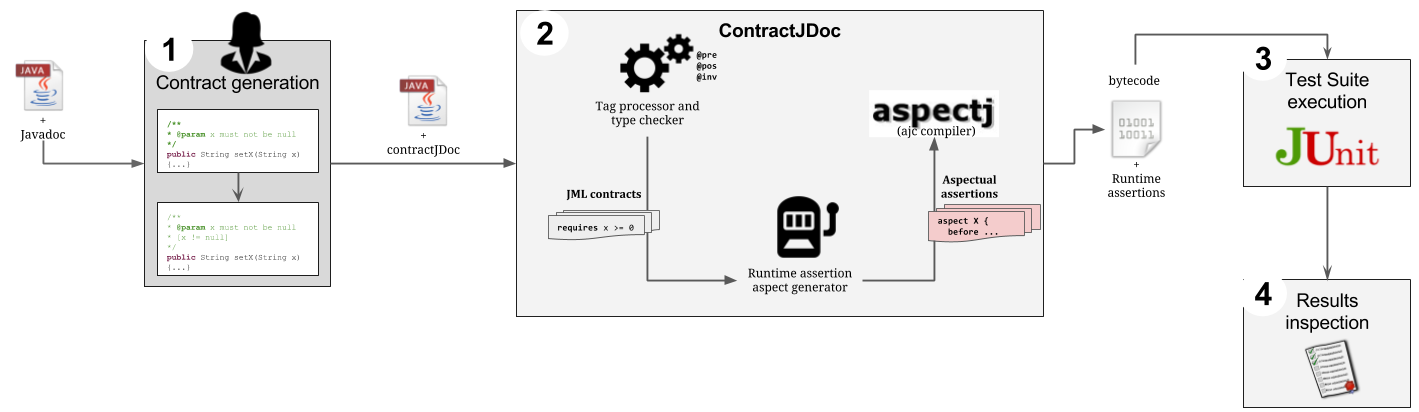
\includegraphics[width=1.0\textwidth]{figs/ContractJDocProcess}
\caption{Steps for applying \contractjdoc{} to Javadoc-annotated systems.}
\label{fig:applicationProcess}
\end{figure}

%contract classification
Concerning the types of external contracts, we group the contracts according to
the approach introduced by XXXXX et al.~\cite{typeContracts}: application-specific contracts
(AppSpec.) -- the kind of contracts that enforce richer semantic properties;
% implications)
 common-case contracts (Com.Case) -- the kind of contracts that enforce
expected (common) program properties;
% methods do not modify unrelated variables; 
code-repetitive (Repet.) -- the kind of
contracts that repeat exact statements from the code.
% : that a method returns a

%experiment package - link
All systems used in this study are available in a replication
package.\footnote{\url{https://goo.gl/yO8or2}; in order to run the
\contractjdoc{} compiler, the folder \textit{aspectjml-lib} must be copied into the folder of each system.}
%when we consider an error
Concerning the verification performed after applying \contractjdoc{} contracts into the systems,
we used the test suites available with the purpose of identifying problems
(four out of \totalSystems{} projects have a test suite available).
Every test case that failed was investigated in order to find out if it was a conformance error in the system.

% applying dbcjdoc
As a secondary goal, the study allowed us to check the expressiveness of \contractjdoc{} and to
evaluate the effort related to adding contracts to existing systems.
In addition, we enhanced the compiler and added features in order to simplify
the process of applying \contractjdoc{} in existing projects.


\section{Results}
\label{sec:results}

We start by describing the results for each study in detail, before proceeding to summarise and discuss the observed effects.

\subsection{Experimental Simulation}
\label{sec:expResults}

%demographics
The selected participant set encompasses graduates in Computer Science or Software Engineering -- either working in industry (41.6\%) or M.Sc. and Ph.D. candidates (58.4\%).
%table
In Table~\ref{tab:results} we summarise the results from the 24 trials, from which five -- 21\% -- were delivered with at least one fault detected by our test cases.
%individual results
All participants assigned to textual specifications in Javadoc delivered correct programs.
By contrast, half of the programs delivered by participants using APIs with formal contracts were faulty (four out of eight).
One faulty program was delivered by a participant from the \contractjdoc{} group.
%task
Regarding task, faulty programs were mostly present in API implementations -- four of them, if compared with only one in API clients.


% source code correct
%Javadoc and \contractjdoc{} were the only documenting approaches in which all participants were able to produce a code satisfying the oracle (respecting the restrictions available in the comments). On the other hand, there was one case developed by following the JML documenting approach in which the contract is not satisfied by the implementation.



\begin{table}
\centering
\caption{Experimental results, for each treatment (textual Javadoc \emph{JavaDoc}, \contractjdoc{} \emph{ContJDoc} and formal contracts \emph{Formal}. For each API (Queue or Stack) and Task (\emph{Cli} if a client for the API was implemented, \emph{Sup} if an implementation for the API was provided), participants are listed (\emph{Part}) along with the result (\emph{Res}) from our test cases.}
\label{tab:results}
\begin{tabular}{|l|l||l|l||l|l||l|l|} 
\cline{3-8}
\multicolumn{1}{l}{} &              & \multicolumn{2}{l||}{\textbf{JavaDoc }} & \multicolumn{2}{l||}{\textbf{ContJDoc }} & \multicolumn{2}{l|}{\textbf{Formal}}  \\ 
\hline
\uline{DataStr}      & \uline{Task} & Part & Res                              & Part & Res                                & Part & Res                             \\ 
\hline\hline
\uline{Queue}        & \uline{Cli}  & p9   & \greencheck       & p11  & \greencheck                                    & p7   & \greencheck                                 \\
                     & \uline{Cli}  & p10  & \greencheck                                 & p12  & \greencheck                                    & p8   & \greencheck                                \\
                     & \uline{Sup}  & p21  & \greencheck                                 & p23  & \greencheck                                    & p19  &  \greencheck                               \\
                     & \uline{Sup}  & p22  & \greencheck                                 & p24  & \greencheck                                    & p20  &  \redcross                               \\ 
\hline\hline
\uline{Stack}        & \uline{Cli}  & p3   & \greencheck                                 & p5   & \greencheck                                    & p1   & \redcross                                 \\
                     & \uline{Cli}  & p4   & \greencheck                                 & p6   & \greencheck                                    & p2   & \greencheck                                 \\
                     & \uline{Sup}  & p15  & \greencheck                                 & p17  & \redcross                                    & p13  & \redcross                                \\
                     & \uline{Sup}  & p16  & \greencheck                                 & p18  & \greencheck                                    & p14  & \redcross                                \\
\hline
\end{tabular}
\end{table}

%faults
Table~\ref{tab:faults} details the faults detected by the test cases. After a detailed analysis of the programs, we classified each fault regarding the violated contract. 
%clients
All clients fulfilled the specified pre-conditions for calling API methods -- p1's client raises an exception which was incompatible with the method's post-condition.
%suppliers
All four faults unveiled in API implementations resulted from failing to satisfy the specified post-condition in methods removing data from the given structure (two on \texttt{Stack.pop} and two on \texttt{Queue.remove}).

\begin{table}
\centering
\caption{Reason (fault) for failures in participants' results}
\label{tab:faults}
\begin{adjustbox}{width=\textwidth}
\begin{tabular}{|l|l|l|l|} 
\hline
\multicolumn{4}{|l|}{\textbf{ContractJDoc }}                                                                                                                                                                    \\ 
\hline
p17                                        & Stack                             & Sup                                & Post-condition violation on method \texttt{remove}                                    \\ 
\hline
\multicolumn{4}{|l|}{\textbf{Formal contracts} }                                                                                                                                                                \\ 
\hline
p1                                         & Stack                             & Cli                                & Failure to expect correct exceptions from Post-condition on method \texttt{removeAccountTop}    \\ 
\hline
p13                                        & Stack                             & Sup                                & Post-condition violation on method \texttt{pop}     \\ 
\hline
p14                                        & Stack                             & Sup                                & Post-condition violation on method \texttt{pop}     \\ 
\hline
p20                                        & Queue                             & Sup                                & Post-condition violation on method \texttt{remove}  \\ 
\hline\hline
\multicolumn{1}{|c|}{\textbf{Part}} & \multicolumn{1}{c|}{\textbf{API}} & \multicolumn{1}{c|}{\textbf{Task}} & \multicolumn{1}{c|}{\textbf{Type of~Fault}}                                               \\
\hline
\end{tabular}
\end{adjustbox}
\end{table}

After they sent their code back, we asked participants about understandability of the API specifications, using a Likert-like scale which ranges from 1 (less understandable) to 5 (very understandable). The results for 24 answers are summarised in Figure~\ref{fig:ExpAnswersTotal}, in which assessments are spread between 3 to 5. Most participants evaluated understandability as 4 (58\%).

\begin{figure*}
\centering
\begin{subfigure}{.32\textwidth}
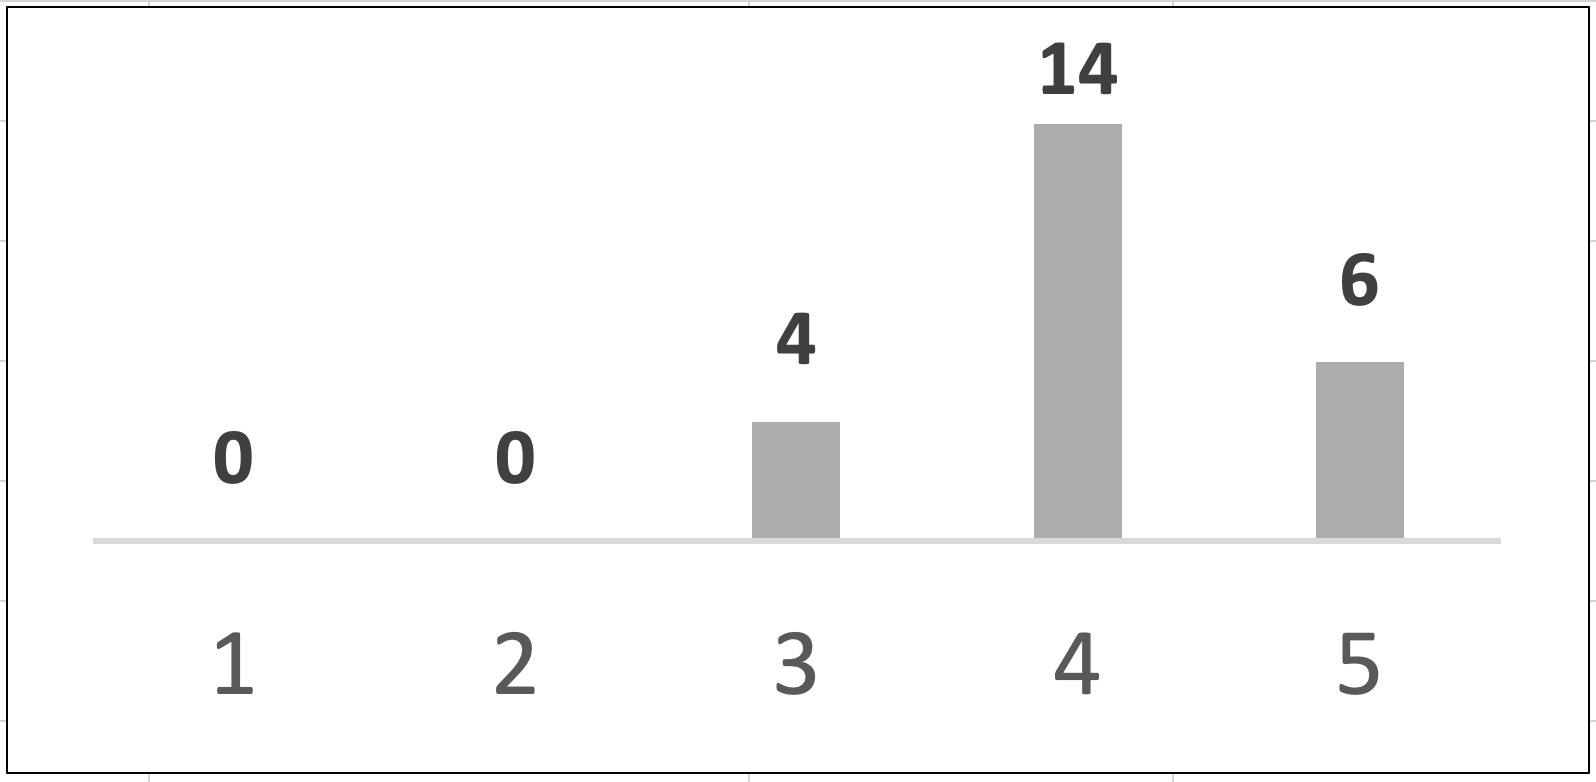
\includegraphics[width=1\textwidth]{figs/ExpAnswersTotal.png}
\caption{Total Results.}
\label{fig:ExpAnswersTotal}
\end{subfigure}
\begin{subfigure}{.33\textwidth}
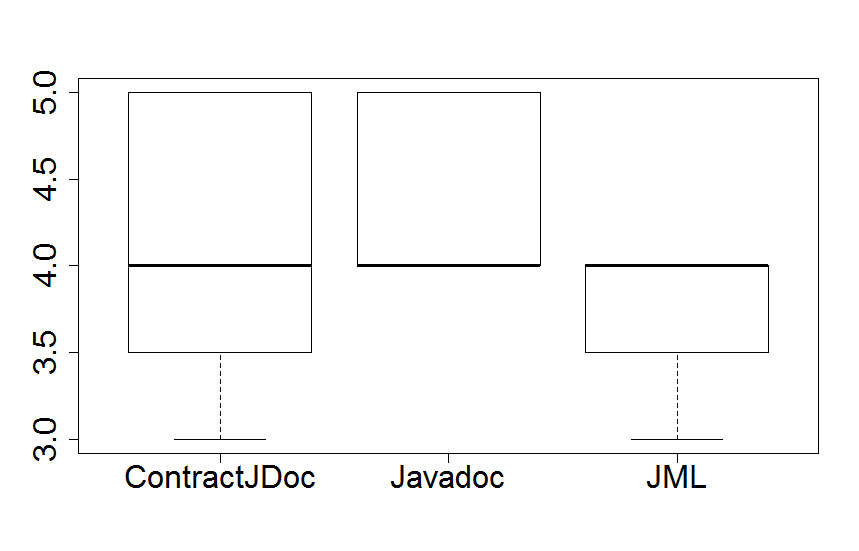
\includegraphics[width=1\linewidth]{figs/boxplotApproachesEmpiricalStudy}
\caption{Results by approach.}
\label{fig:approachesEmpirical}
\end{subfigure}
\begin{subfigure}{.33\textwidth}
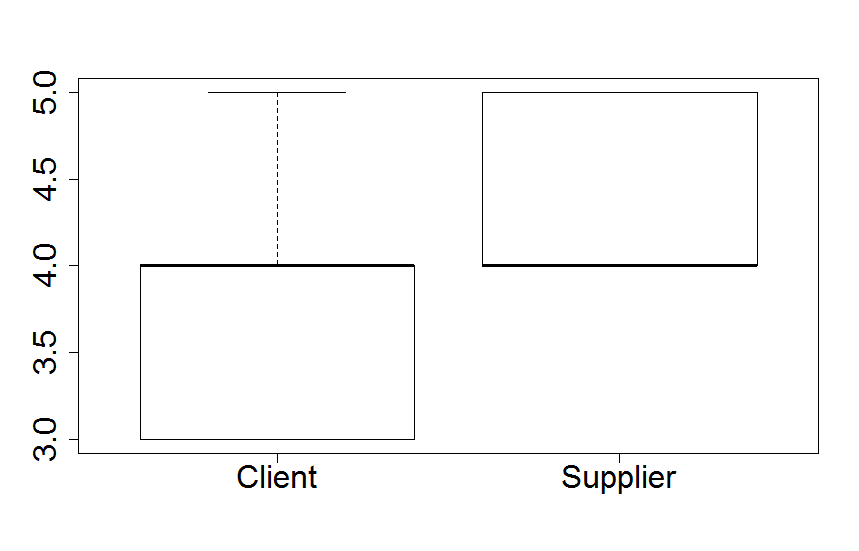
\includegraphics[width=1\linewidth]{figs/boxplotTasksEmpiricalStudy}
\caption{Results by task.}
\label{fig:tasksEmpirical}
\end{subfigure}
\caption{Results from Understandability Assessment of API specifications, as Perceived from Participants.}
\label{fig:empiricalResults}
\end{figure*}

%perspectives
Assuming a distinct perspective, we grouped understandability assessments by the assigned documentation approach and task -- Figures~\ref{fig:approachesEmpirical} and~\ref{fig:tasksEmpirical}, respectively, depict their distribution using boxplots.
%doc approach
Visually, the assessments for Javadoc APIs are all above the median ($4$), while \contractjdoc{} assessments fluctuate around that median value. Formal contracts, in turn, were all assessed as $3$ or $4$.  
% stats
Nevertheless, statistical tests (in this case, the Kruskal-Wallis non-parametric test) showed no difference between the groups (p-value = $0.15$, 95\% confidence level).

%task
Concerning the task performed by the developers, higher understandability is reported by participants assigned to supplier tasks, at least visually. Still, the Wilcoxon rank sum test~\cite{statistical} reported no significant difference (p-value = 0.07, for confidence level of 95\%).

%qualitative results
Furthermore, we asked the participants, with an open-ended question, to provide comments on their tasks.
The quotes were organised in 11 categories, which are presented in Table~\ref{tab:categories}, in conjunction with the number of quotes. One quote might be classified in more than one category -- three participants did not provide an answer.

%on the results
%seven
We found that most quotes either value the specifications or suggest the contracts should have been stronger (seven each). As an example of the latter, p6, which was assigned a \contractjdoc{} API, wrote: "I hesitated over the \texttt{pop} method, due to its exception; there should be more information about the exception to be thrown in each case". 
%four
Others made explicit suggestions on how the specification should be, from their previous understanding of Queue and Stack APIs.
%other
Interestingly, we found a few quotes that expressed total trust in the contracts, dismissing defensive programming as advocated by the Design by Contract methodology ~\cite{dbc}.
Another category encompasses quotes that remark how the Javadoc text around the contract expressions helped them to understand the API specification. 

\begin{table}
\centering
\caption{Categories in Participants' quotes}
\label{tab:categories}
\begin{tabular}{|l|r|} 
\hline
\textbf{Category description}                & \multicolumn{1}{l|}{\textbf{\#quotes}}  \\ 
\hline\hline
Specifications were clear and understandable & 7                                       \\ 
\hline
Specifications were vague                    & 7                                       \\ 
\hline
Suggestions to change the specification      & 4                                       \\ 
\hline
The surrounding text helped understanding    & 2                                       \\ 
\hline
Total trust in the contracts                 & 2                                       \\ 
\hline
Contracts were ignored                       & 1                                       \\ 
\hline
Hard to read the logic                       & 1                                       \\ 
\hline
Questions about the task                     & 1                                       \\ 
\hline
Text was confusing                           & 1                                       \\
\hline
\end{tabular}
\end{table}


\subsection{Judgment Survey}
\label{sec:surveyResults}

%survey description
As a follow-up for the lab study, we showed three versions of the Stack API as a web survey, asking questions about those approaches to contract specifications; we suggested respondents play the client role of the API as if they were about to instantiate it and call its methods.
%questions
Respondents were asked to assess understandability of each approach (again, using a 1--5 Likert scale), in addition to providing a verdict asking which approach they think is the most understandable as an API specification. For this, they were given three options -- one for each approach -- and a fourth, neutral option.

%general results
From the universe of developers who received the invitation, answers from 142 Java developers were considered valid.
%demographics
%students and professionals
From those, 51 are graduate professionals (36\%), and 91 are undergraduate and graduate students in computer-related degrees (64\%).
%experience
Having some experience with Java was a requirement for being a participant; more than 73\% (105) have experience with either open source or industrial projects. Likewise, 74\% (105) of the respondents declared to have more than one year of Java programming.
%contract experience.
Regarding formal contract languages for specifying APIs (Eiffel, JML or similar), most respondents -- 67\% -- had no previous experience. 


%results - Javadoc is the simplest
Concerning the survey answers, it is shown in Figure
~\ref{fig:mostUnderstandable} that 50.7\% (72) of the respondents chose Javadoc as the most straightforward approach to understanding the provided API specification. 
%contractjdoc em JML
While only 11 (7\%) chose formal contracts as the most understandable approach and 18 (12\%) were indifferent, an almost one-third of the respondents (41, almost 29\%) chose the mix of text and contract expressions -- \contractjdoc{}.


\begin{figure}
\centering
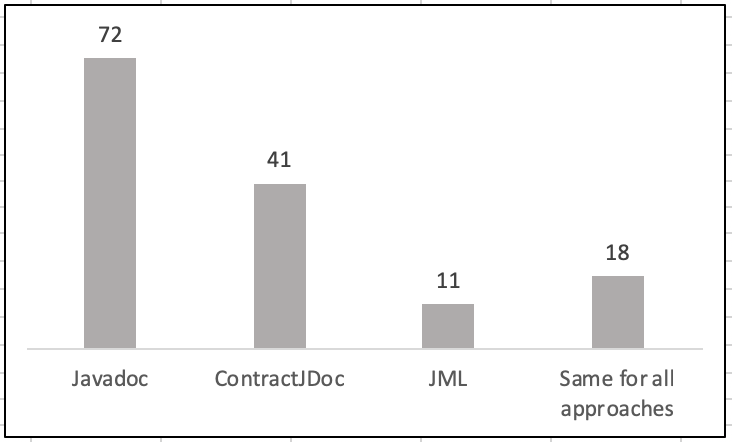
\includegraphics[width=0.7\linewidth]{figs/mostUnderstandable.png}
\label{fig:mostUnderstandable}
\caption{Surveyed Verdicts on the Most Understandable Contract Style.}
\end{figure}


% individual answers to each approach
After being presented with three versions of the same API, the distribution of assessments for each documentation approach is showed in Figure~\ref{fig:allApproaches}.
%explain visual
Answers for Javadoc and \contractjdoc{} were distributed around a median of $4.0$; for the first, assessments range from $3$ to $5$, while assesments for the latter were no higher than $4$.
Likewise, formal contracts were evaluated with $4$ the highest, however with $3$ with centre value. 

\begin{figure}
\centering
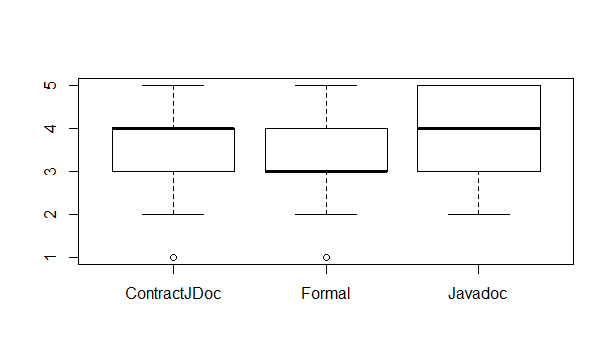
\includegraphics[width=0.7\linewidth]{figs/boxplotApproachesSurveyStudy}
\caption{Surveyed Assessment for Each Documentation Approach.}
\label{fig:surveyResults}
\end{figure}


%statistical results
Differently from the experimental simulation from Section~\ref{sec:expResults}, statistical tests show a significant difference between the assessments. The application of One-way ANOVA, which is robust enough for non-normal distributions~\cite{statistical}, detected a distinction between the three groups of answers (p-value $<$ 0.05). A corresponding post hoc analysis -- Tukey HSD 
%and pairwise comparisons using t tests
with Bonferroni correction~\cite{statistical} produced the following p-values for each pairwise comparison: Javadoc-ContractJDoc = 0.012, Formal-ContractJDoc = 0.000, and Formal-Javadoc = 0.000. The results then express the significant difference between all styles.
%effect sizes


%When analysing data grouped by experience (Figures~\ref{fig:javadocExp} to~\ref{fig:jmlExp}) using Wilcoxon rank sum test with continuity correctiontests, only for JML we found no statistical difference between Professionals and Students (p-value = 0.17). For both Javadoc and \contractjdoc{}, Professionals had perceived the approaches as being easier for comprehensing than Students (p-value = 0.012 and p-value = 0.004, respectively).


\subsection{Case Study}

Table~\ref{tab:caseStudyResults} exhibits the results of translating real Javadoc specifications to \contractjdoc{} in each system.
%columns
Column \textbf{Faults} presents the failures raised by the original test suite (whose size is showed in Column \textbf{TCs}), with source code enhanced by \contractjdoc{}, while Column \textbf{Time} measures the seconds spent in compiling the system instrumented with \contractjdoc{} before running the test cases. 
%MASSONI: confirmar isso acima.
\textbf{Clauses} displays how many contract clauses were translated into contract expressions, which are classified -- according to XXX et al.~\cite{typeContracts} -- in Columns \textbf{CommCase}, \textbf{AppSpec} and \textbf{Repet}.

\begin{table}
\centering
\caption{Results from Study Replacing Javadoc with \contractjdoc{}.}
\label{tab:caseStudyResults}
\begin{adjustbox}{width=\textwidth}
\begin{tabular}{lrrrrrrr} 
\hline
\multicolumn{1}{l}{\textbf{System}} & \textbf{Faults} & \textbf{Time(s)} & \textbf{TCs}     & \textbf{Clauses}                          & \textbf{CommCase} & \textbf{AppSpec} & \textbf{Repet}  \\ 
\hline
Dishevelled       & 381                                 & 434                                     & 2,643                            & 2,655                                     & 1,536                                  & 151                                    & 968                                   \\
Webprotégé      & 0                                   & 713                                     & 0                                & 930                                       & 717                                    & 282                                    & 1,214                                 \\
ABC-Music-Player  & 2                                   & 14                                      & 30                               & 115                                       & 42                                     & 11                                     & 62                                    \\
Jenerics          & 7                                   & 20                                      & 44                               & 190                                       & 156                                    & 0                                      & 34                                    \\
OOP Aufgabe3      & 1                                   & 4                                       & 11                               & 54                                        & 16                                     & 30                                     & 8                                     \\
%MASSONI: ELIMINEI SimpleShop
% SimpleShop        & 0                                   & 5                                       & 0                                & 50                                        & 30                                     & 11                                     & 9                                     \\
\bottomrule
\textbf{ Total }  & \textbf{391}                      & \textbf{1,185}                        & \textbf{ 2,728 }                 & \textbf{\totalClauses{}} & \textbf{ 2,497 }                       & \textbf{ 282 }                         & \textbf{ 1,214}                       \\
\bottomrule
\end{tabular}
\end{adjustbox}
\end{table}


% \begin{table*}[h]
% \caption{Results from Applying \contractjdoc{} Replacing Javadoc.}
% \label{tab:caseStudyResults}
% \centering
% \begin{tabular}{l l l l l l l l}
% \hline
%  \bfseries System &
%  \bfseries \#Clauses & 
%  \bfseries \#Errors & 
%  \bfseries Time (s) &
%  \bfseries \#Tests &
%  \bfseries \#Com.Case &
%  \bfseries \#AppSpec. &
%  \bfseries \#Repet. \\ \hline
% ABC-Music-Player & 115 & 2 & 14 & 30 & 42 & 11 & 62 \\
% Dishevelled & 2,655 & 381 & 434 & 2,643 & 1,536 & 151 & 968 \\
% Jenerics & 190 & 7 & 20 & 44 & 156 & 0 & 34 \\
% OOP Aufgabe3 & 54 & 1 & 4 & 11 & 16 & 30 & 8 \\
% SimpleShop & 50 & 0 & 5 & 0 & 30 & 11 & 9 \\
% Webprot\'{e}g\'{e} & 930 & 0 & 713 & 0 & 717 & 79 & 133 \\ \hline

%  \bfseries Total & 
%  \bfseries \totalClauses{} & 
%  \bfseries 391 &
%  \bfseries 1,185 &
%  \bfseries 2,728 &
%  \bfseries 2,497 &
%  \bfseries 282 &
%  \bfseries 1,214
% \\
% \bottomrule
% \end{tabular}
% \end{table*}


%commentary on the table
From the selection of open source systems, only \emph{WebProtégé}'s test suites were unavailable; we translated their clauses nonetheless due to the richness of its Javadoc specification.
The size of the available test suites is proportional to the system size.
\emph{Dishevelled} is much larger than the other selected systems, naturally presenting a higher rate of anomalies, which provided us with an abundant source of analysis about the mismatches between specification and implementation. 
%MASSONI: temos o tempo que cada sistema usou pra compilar SEM A INSTRUMENTACAO?
About the time...



% results for contract types
Concerning the kind of contracts, the only unit for which we wrote more application-specific contracts was the \emph{OOP Aufgabe3} system (55\% of the written contracts are application-specific). On the other hand, in \emph{ABC-Music-Player}, more than 90\% of the contracts remain between common-case and repetitive code: verifications that strings are not blank, collections are not empty, or that a method returns a field.
For \emph{Dishevelled}, most contracts are classified as common-case (57.51\%) -- 
%other 36.92\% are repetitive with code and 
only 5.57\% are application-specific.
Similarly, all contracts written for \emph{Jenerics} are related to verification of nullity from parameters or the return value, thus all contracts
remains between common-case and repetitive code.
For \emph{WebProt\'{e}g\'{e}}  common-case contract expressions amount to 77.51\%.  

%In \emph{SimpleShop}, the written contracts are distributed in the following manner: common-case 60\%, repetitive code 19\%, and application-specific 21\%; again the number of common-case and repetitive code outperforms application-specific contracts. 


\section{Discussion}
\label{discussion}

This section comprises discussion on the results from our empirical studies: experimental simulation, judgment survey and case study -- using, as basis, the aforementioned research questions, and threats to validity.


\subsection{RQ1. What is the Effect of the Documentation Approach on API Usage and Implementation Tasks?}
\label{rq1}

%code correctness, each approach
Concerning code correctness, all participants assigned to Javadoc APIs produced code
in accordance with the contracts -- our manually-produced test cases did not detect any contract violation. One \contractjdoc{} API implementation was delivered with a single fault, while half of the participants assigned to API with formal contracts presented at least one fault.
%problems in understanding formal contracts
These results may suggest participants had trouble understanding API formal contracts, assuming their self-reported experience in Java programming and their intention to complete the assignment correctly.
%no test cases
Since we did not provide our test cases, participants were asked to test at their discretion, and failure in fulfilling contracts as specified was not detected by them.
%at least one example
For example, we established the following postcondition for \texttt{Queue.remove}, using a JML-like notation
\begin{lstlisting}[basicstyle=\footnotesize\ttfamily,name=figxpi, frame=lines, mathescape=true]
/**
   
\end{lstlisting}
p20's submission presented an implementation to \texttt{remove} \ldots 

%reports from faulty participants
Surprisingly, no participant assigned to formal contracts reported any problems in their subjective answer –– p13 and p20 suggested changes to contracts, arguing they were vague and should be made stronger, while p14 asked a simple question about the task; p1 even reported "the documentation and contracts (\ldots) are clear".
%discussion 
Even though developers understand the relevance of API formal contracts for the task, they may have misinterpreted the expected behavior, violating it with their implementation.
In order to avoid such scenario, some sort of automatic verification would be critical.
Since research has showed that developers often resist in applying formal specifications~\cite{}, contract expressions amid textual specifications might be useful.

%the only error in cjdoc
p17 -- the only participant assigned to \contractjdoc{} whose implementation violated a contract clause -- remarked he/she "\emph{trusted the contract expressions}", 
%issue - forgetting the contract!
which raises the issue of, by rejecting defensive programming~\cite{}, one failing to notice contract restrictions, such as a basic assumption to ensure a post-condition clause.
%solution?
Again, test cases specific to the contract expressions should have made it easier to detect the nonconformance.

%in our case
Four of those faults were submitted by implementers, which might be predictably more common, as API Clients could rely on simple tests or even additional compilation checks for not adding faults like the one added by p1.
%This example also illustrates that trivial misunderstandings like this would often go unnoticed if specifications were only textual.  
%another explanation
This outcome may also be explained by the awareness required in using methods provided by the API: one needs to read the documentation available in order to know how to use the methods, whereas implemention could be considered more straightforward -- in this simulation, 
the APIs make up well-known data structures, thus their specifications may have been neglected -- although none of the participants' comments explicitly evidence this speculation.

%types of faults
All faults in the experiment failed to ensure post-conditions. 
%postcond are harder
Studies show these contracts are the trickier to write~\cite{}, and, by extension, might be also harder to follow (by API Clients) or fulfill (by API implementers). 
%no preconditions!
It is also noticeable that no pre-condition violations were detected. We might speculate that, because pre-conditions are the most commonly used type of API contract~\cite{}, developers are likely to be concerned about fulfilling them from the start. 
Pre-conditions might be as well a deliverance to developers in two ways: API clients are inclined to comply right way, before calling any method, so they soon accomplish their contract obligation; and API implementers can assume the pre-condition for neglecting defensive programming, writing thus less code.

%problems with kinds of contract
Furthermore, qualitative data from participants do not present any reported issues with pre-conditions -- eight quotes are, as a matter of fact, \emph{compliments} to their clarity. On the other hand, nine participants make at least one remark about the trouble in understanding or accepting the post-conditions as they were provided.



\subsection{RQ2. What is the Effect of the Documentation Approach on the Understanbility of API Specifications?}
\label{rq2}

%all results
From the assessments by the participants in our experiment, no statistical effect was perceived in using either of the three approaches. All participants, in fact, perceived all API specifications as having medium to high understandability (Figure~\ref{fig:ExpAnswersTotal}). 

%first conclusion
Nevertheless, by analyzing the assessments in together with the provided qualitative data, we notice a trend: Javadoc as the top approach and formal contracts as the least understandable approach. The \contractjdoc{} approach, mixing Javadoc and contract expressions, was assessed as intermediate, which is illustrated in Figure~\ref{fig:approachesEmpirical}.
%expected
This outcome is expected, as developers tend to favour informal styles for documentation -- a known obstacle for the adoption of DBC~\cite{}. In such scenarios, the approach employed in \contractjdoc{} is promising for a more gradual adoption of DBC in mainstream programming languages like Java.

%conclusion from survey
Reinforcing this conclusion, the judgement survey with 142 respondents analogous results. 
In this case, however, differences between all groups are statistically significant -- in detail, (effect sizes and pairwise) /ldots
Larger effect sizes when formal contracts are compared with either Javadoc and \contractjdoc{}, and a smaller effect size between Javadoc and \contractjdoc{} (higher understandability for the first).
%more on the answers
\contractjdoc{} was considered understandable for 75\% of the answers, if regard as such assessments $4$ and $5$.

%back to experiment, 
Turning our attention back to experimental simulation data, participants reported higher understandability of API specifications when they were assigned to its implementation. Nevertheless, more submitted API implementations were faulty, in comparison to API clients (Table~\ref{tab:faults}). 
%conclusion
We then could possibly infer that the relationship between the perceived understandability and actual outcome of using API contracts might be orthogonal, although statistical evidence is absent for a more credible conclusion. 


\subsection{RQ3. What Kinds of Nonconformances can be Uncovered if Javadoc Specifications are Replaced by Contract Expressions?}
\label{rq3}


% applying contractjdoc
For all systems (see Table~\ref{tab:Units}), we
wrote more pre- and postconditions than invariants. This result has two
explanations: first, as expected the amount of Javadoc comments over the
classes' fields in the evaluated systems is low in comparison with the amount
of Javadoc comments over method's parameters and return.
Those results corroborate with other research~\cite{} 


%  -- the only
% exception occurred in \texttt{SimpleShop} system because the developers have used resources from Java
% constraints for declaring some fields as not null, enabling us to establish
% invariants for them; second, even when there are no comments in a method, we are
% able to write pre- and postconditions based on analysis of method's body.

Data needed here: number of pre-, post-, invs- \ldots

Concerning pre- and postconditions, for \texttt{ABC-Music-Player} and
\texttt{WebProt\'{e}g\'{e}} projects, we wrote almost twice as many postconditions
as preconditions.
In \texttt{ABC-Music-Player} this is related to the number of accessor methods
available and for \texttt{WebProt\'{e}g\'{e}}, the difference is related to
the available comments.



%  and to the contracts we are able to infer from method's
% body.
%
% In addition, based on the comment and the body of a method, establishing a
% postcondition appears to be simpler than a precondition, as we do not know
% the methods' clients beforehand.


Data needed here: number of violations for each of two groupings:
(1. by pre-, post-, inv-)
(2. CommCase, AppSpec, Repet.)
One paragraph of discussion for each.


%exceptions in ABC-MUSIC-PLAYER

\textbf{Add Example. }
We were able to detect potential inconsistencies in \texttt{ABC-Mu\-sic-Player};
the exception will be always thrown, differently from what is expected from the
commentary.
We also found a problem into
\texttt{WebProt\'{e}g\'{e}} project, in the class \texttt{OWLLiteralParser} there was one exception
in the Javadoc tag \texttt{@throws} that was not declared in the throws of the method's signature.

% conformance errors
\textbf{Add Examples. }
In addition, sometimes the tests available along with the systems do
not respect the definitions from the Javadoc comments. For instance, when the
comments in natural language from \texttt{ABC-Music-Player} system are turned into
\contractjdoc{} contracts, some tests from
\texttt{MainTest}, \texttt{ParserTest}, and \texttt{SequencePlayerTest} violate
the methods' preconditions from class \texttt{Utilities}, they try to
call \texttt{Utilities}' methods by passing the value zero as the second
parameter, even though the comment declares the second parameter must be greater than zero.
This scenario also occurred in \texttt{Dishevelled} unit, the comments turned
in \contractjdoc{} contracts also enable us to detect some tests
that do not respect the restrictions available in the Javadoc comments.


% conformance errors
\textbf{Add Examples. }
When applying \contractjdoc{} to \texttt{ABC-Music-Player}, we found inconsistencies between Javadoc comments and the source code. The problems occurred in the class \texttt{Utilities} (package
\texttt{sound}) because there are comments concerning a parameter declaring that the value of
this parameter must not be greater than or equal to zero; however in the body of the methods there
is an if-clause that throws exceptions when the value received by the parameter is negative.
\textbf{Discuss open source software evolution, with citations}.

%final conclusion
As a proof of concept, \contractjdoc{} and its compiler (\contractjdocCompiler{}) enabled us to write runtime
checkable code for third-party systems based on the comments in natural
language.
As expected, the quality and variety of the contracts depended strongly on the available comments, however, we were able to
detect and correct inconsistencies and missing expressions between source code and comments.




\subsection{Limitations and Threats to validity}
\label{sec:CaseStudyThreats}

%external validity
External validity refers to generalization. Due to its size, results from the
case study cannot be generalized; its purpose is evaluating applicability and relative usefulness.
%represetantive sample
The sample is not representative, since there is no available estimate of the Javadoc-rich project
population in GitHub, then probability sample is impossible.
Our approach is as systematic as feasible in selecting the evaluated project -- manual translation
does not scale, then the sample contains only \totalSystems{} projects.
Therefore, those systems may not be representative of the real use of Javadoc in real systems; however, we were able
to detect inconsistencies between Javadoc comments and source code, as occurred in
\texttt{Utilities} class (\texttt{ABC-Music-Player} experimental unit) in which the comment for a
parameter of the methods is the right opposite of the expected behavior in the source code.


%external
Another risk is that only 24 developers participated in the experimental study
and 142 in the survey and those samples are not representative for the community
of Java developers. Furthermore, we used only two similar data structure interfaces (queue and stack). In other domains with more complex structures, the results
may vary. In addition, the survey used only one data structure interface:
\texttt{Stack}, for asking about the comprehensibility of the interface behavior.
In other domains with more complex structures, the results can vary considerably.


%internal
Internal validity refers to causation: are changes in the dependent variable
necessarily the result of manipulations to treatments? All material for the
empirical study and the survey study is available only in English, therefore,
the experience of the Subject with English can have affected their
comprehensibility of the behavior of the provided interface.

%construct
Construct validity refers to correctly measuring the
dependent variable. \texttt{Dishevelled} and
\texttt{WebProt\'{e}g\'{e}} sizes set them apart from the other systems.
For instance, \texttt{Dishevelled} is more than 56 times bigger than \texttt{ABC-Music-Player}, 43
times bigger than \texttt{Jenerics}, 313 times bigger than \texttt{OOP Aufgabe3}, and 234 times
bigger than \texttt{SimpleShop}.
In order to reduce the threat on the manually-defined contracts,
all systems were annotated and reviewed by three researchers, separately.


The order in which we display the documented
interfaces on the survey form, the questions used for evaluating
comprehensibility, the kind of questions used, and the absence of opened questions
can also threat the construct validity. For dealing with these threats we
perform a pilot before applying the survey and used the results from the pilot
to improve the survey structure. In addition, the answers from developers may not be
representative of their real opinion on difficulty perception; to overcome this
threat we made a space for comments available along with the Likert-scale
questions, which are taken into account when collecting the answers.

\section{Related Work}
\label{sec:relatedWork}

\textbf{Contracts.} 
As discussed, each contract-based approach choo\-ses a different trade-off between expressivity/preciseness, verbosity, freedom, and tooling (e.g., runtime checking).
This is the case of JML~\cite{jml} and Microsoft's Code Contracts~\cite{codeContractsPaper}.
Both enable one to provide full behavioral specifications and their runtime checking.
Nevertheless, they lack support to allow informal specifications or to be available at third-party
library clients~\cite{Parnas2011}. They differ in the way they are written; the former is written as Java comments in code, whereas the latter is syntax-based and therefore often verbose. 
Without tool support to extract meaningful specifications the contracts provided by Code Contracts are even less interesting for third-party libraries, since they are embedded in C\# programs. Differently from these languages, the contracts expressed in \contractjdoc{} are already embedded in Javadoc comments, which are the standard approach to documenting Java programs and more likely to be available to third-party libraries.

%ecoop2017
Recent work by Dietrich et al.~\cite{Dietrich2017} catalogued 25 techniques, found within the code of 170 open-source systems, that are considered contracts. They include specialized constructs such as the ones offered by JUnit (e.g., \texttt{assertNotNull}), java asserts within the code itself, \emph{ad hoc} methods with exceptions (e.g., Java \texttt{IllegalArgumentException}), in addition to external contract libraries, such as Guava). 
Their approach is based on the assumption that developers are more likely to adopt simpler forms of contracts, such as type annotations and assertions. The notion of contracts respects "the general assume-guarantee principle and follows the \emph{Design by Contract} viewpoint promoted by Meyer, where contracts are viewed as lightweight specifications."~\cite{dbc} 

Regardless of their use as lightweight runtime assertions, software designers may as well apply contracts as specification assets for APIs. Several applications of contracts promote them as relevant pieces of information for routines' users~\cite{docAnalysis}. For instance, Java asserts cannot be used as preconditions. Most constructs considered as lightweight contracts (runtime exceptions, Guava, Apache and Spring APIs, Java asserts) can only be found within methods' implementations, thus not amenable for API documentation, as we focus on this paper.

In consonance with our studies, the authors observe a prevalence of pre-conditions over post-conditions; suggested reasons for this result include library code reuse, in which modern libraries have to provide defensive APIs to deal with unknown clients. Given a large portion of the sample projects consists of APIs, most of the contracts are likely to be found in Javadoc commentary, which means that \contractjdoc{}, if used, could increase this number considerably.

\textbf{Javadoc Comments.}
@TCOMMENT~\cite{atComment} is an approach for testing Javadoc comments, specifically method properties about null values and related exceptions. The approach consists of two components: the first component takes as input source files for a Java project and automatically analyzes the English text in Javadoc comments to
infer a set of likely properties for a method in the files; the second component generates random tests for these methods, checks the inferred properties, and reports inconsistencies. By using
\contractjdoc{}, a developer is able to write contracts richer than those for checking null values and exceptions (as presented in Section~\ref{sec:caseStudy}).

Zhai et al.~\cite{docAnalysis} present a technique that builds models for Java API functions by analyzing the documentation. Their models are simpler implementations in Java compared to the original ones and hence easier to analyze. More importantly, they provide the same functionalities as the original functions. They argue that API documentation, like Javadoc and .NET documentation, usually contains wealthy information about the library functions, such as the behavior and exceptions they may throw. Thus it is feasible to generate models for library functions from such API documentation. In this context, the comments in \contractjdoc{} approach can be used as input for the technique in order to improve model generation.

% \textbf{Testing.}
% Clousot~\cite{clousot} statically checks C\#/Code
% Contracts programs. The approach is based on abstract interpretation and analyzes annotated programs
% to infer facts (including loop invariants), and it uses this information to discharge proof
% obligations. 
% AutoTest~\cite{autotest} is a collection of tools that automate the testing process for
% Eiffel programs. In AutoTest, contracts are used as oracles to expected outputs for conformance checking of the programs; furthermore, AutoTest uses a randomly-guided tests generation (ARTOO~\cite{artoo}) and
% supports mixing manual and automated test. 
% \jmloktool{}~\cite{jmlok2} is a tool for dynamically detecting and classifying nonconformances in contract-based programs, applying randomly-generated tests (RGT) for detecting nonconformances, and a heuristics-based approach for nonconformance classification. 
% These tools are for contract-based languages; in contrast, we propose and implement an approach for writing contracts in the same language as the source code, such as available in JML and Eiffel, improving documentation.

\textbf{Empirical Studies.}
There are three main related empirical studies about contract usage~\cite{typeContracts,Estler-etal14,Chalin06}.
One common conclusion about is that, in practice, developers use simple and short contracts~\cite{typeContracts,Estler-etal14}. For instance, \cite{typeContracts} shows that 75\% of the projects' Code Contracts are checks for the presence of data (e.g., non-null checks).
In our case study (Section~\ref{sec:caseStudy}), almost 93\% (3,711 contract clauses out of 3,994) of the contracts we wrote remains between checks for the presence of data and statements repeating the method's return. 
Also, Chalin studied 84 Eiffel~\cite{eiffel} projects and pointed out that developers are more likely to use contracts in languages that support them natively, like Eiffel~\cite{eiffel} or Code Contracts~\cite{codeContractsPaper}. To support both conclusions, \contractjdoc{}could be used to write simple contracts natively, as usual Javadoc comments.

\section{Conclusions}
\label{sec:conclusions}

%context - tradeoffs are clear
It is well known that software developers are resistant to use formal contracts for public methods; for Java programs, for example, textual Javadoc prevail for documenting API behaviour ~\cite{docAnalysis}.
Javadoc's use is widespread, serves for important purposes -- tools for generating documentation -- but lacks, of course, automatic checking of the program against its specification.
%what we have done
The trade-off between the pragmatics of textual descriptions and formal contracts amenability to automatic analysis is explored in this paper, by three empirical studies.
%evaluation of styles
We evaluated the effect on API usage and implementation tasks of three public contract styles in Java programs: textual Javadoc, JML-like formal contracts, and a third option, a small tag-based extension to Javadoc to express pre- and post-conditions among text and other standard tags, which we call \contractjdoc{}.

%studies
The first and second studies evaluated the effect of specification styles on the efficacy and understandability of contract expressions, either for API implementors or users, through an experimental simulation with 24 recruited participants, and a judgment survey with more than a hundred Java developers.
In the third study, we evaluated the potential of detecting anomalies by manually formalising textual Javadoc contracts from open source Java systems into contract expressions, then checking conformance in runtime.


%first question - effect on the programming task
Participants of our experimental simulation submitted programs either using or implementing one among two simple APIs. A factorial design assigned one of the three specification styles for the API's behaviour -- for repetition purposes, two participants were subject to a single $<style,task,API>$ treatment.
Javadoc and \contractjdoc{} groups were more successful in submitting anomaly-free programs, while half of the formal contract group violated at least one contract clause. 
We speculate, by this outcome and by analysing the qualitative data provided by the participants, that developers, despite their awareness of the specified behaviour, were having trouble in interpreting the expressions.  
Moreover, all anomalies happened with post-conditions, which matches conclusions from previous research~\cite{Estler-etal14,sac2017} perceiving the discomfort when dealing with this kind of contract, in comparison with pre-conditions. 


%second question - effect on understandability
We also used the experimental setting for assessing understandability~\cite{Scalabrino2017} of three contract styles. 
In the answers, Javadoc contracts were regarded as the most understandable, followed by the mixed \contractjdoc{} style and, as the least understandable; nevertheless, those differences were not statistically significant. As a follow-up study, we carried out a judgement survey with 142 Java developers with at least one-year experience, in which the results were the same, this time with significant pairwise-difference effect sizes between all three styles.
This outcome is expected, as developers tend to favour informal styles for documentation~\cite{Polikarpova-etal09}. It remains to be investigated whether an intermediate approach such as \contractjdoc{} is understandable enough for fostering the use of DBC in API specifications.

%third question - can we find anomalies?
Finally, our case study applying contract expressions in open source systems resulted in finding 381 anomalies in a single Javadoc-rich system (\emph{Dishevelled}) and ten more in other three toy systems (\emph{ABC/-Music/-Player, Jenerics and OOP Aufgabe3}), showing the potential of using contract expressions in existing Javadoc specifications.
Other interesting findings about those systems include their preference for post-conditions over pre-conditions, although most contracts were classified as \emph{common case} -- enforcing expected program properties, such as nullable variables.

% future work
%hypothesis for future work
Despite their limitations, we believe the studies presented in this paper prompt the research community to investigate some hypothesis with future enquiry. 
%h: relate perceiving understandability and correct, conforming implementation 
Making sense of the specified behaviour in contracts is undoubtedly a necessary condition to providing a program that conforms to the specification, but it is not sufficient; other forces should be considered, such as tool support, enforcing test cases or even the developer's lack of discipline.  
%h: how freedom to neglect defensive programming could be dangerous for conforming implementations 
Additionally, we could investigate whether contract conformance may be undermined by the omission of defensive programming promoted by Dbc -- as it becomes pointless to add program checks to certain conditions, other important conditions might be neglected. 


%h: how developers react to pre- and post-conditions; pre-conditions are a relief, post-conditions are neglected?
In Dbc -- especially for public contracts --, pre-conditions seem easier to regard and fulfil, if compared to post-conditions. However, post-conditions are probably more fundamental to elaborate and useful contracts~\cite{Rosenblum}. Research could be carried out to test this hypothesis, and investigate the rationale behind the observations.   
%h: what are the reasons for not adopting contracts? one evidence is that they are hard to maintain in sync
Finally, the reason for the low adoption of DbC, at least for formal contracts, must be subject of further consideration. As we could observe in our case study with open-source systems, keeping the specification in sync with the program seems to be the main issue, requiring extra resources often not available in software teams with tight schedules. Automatic generation of contracts from programs~\cite{docAnalysis,atComment} seems a reasonable option to address this issue.  

%improve contractjdoc
For \contractjdoc{}, we intend to improve the tags for considering more complex contract expressions, and carry out more studies on its usability and efficiency, in particular for specifying APIs -- adaptation to other programming languages, such as C\#, would be relatively straightforward. 
For instance, we could add support to \emph{autocomplete}, applying Jaro-Winkler string distance~\cite{jaro,winkler99} as a basis.



% %the language extension
% \contractjdoc{} contracts enable runtime checking by using a language similar to the traditional Javadoc,
% and our compiler (\contractjdocCompiler{}) supports new constructs of Java language, such as the
% features from the Java 8, such as lambda expressions.
% The approach allows the use of Design by Contract~\cite{dbc} in a format closer to
% traditional Javadoc comments. 











% When evaluating \contractjdoc{} we found the
% approach almost as understandable as traditional Javadoc comments, with the
% advantage of being able to check behaviour at runtime.
% When comparing JML with \contractjdoc{}, the latter features less specification
% constructs, although results indicate programmers may feel more comfortable with
% it when writing precise behaviour for methods. 
% Besides, we found evidence
% that \contractjdoc{} is more readable than JML.
% advantages
% Furthermore, as JML contracts, contracts in \contractjdoc{} may be used in place of defensive
% programming, by specifying valid inputs for the methods and shortening the source code.



%% Bibliography
\bibliography{ecoop-2019}

\end{document}

